%*************************************************************
% Master Thesis                                              *
% Ing. Minerva Gabriela Vargas Gleason                       *
%  IAI - Institute of Artificial Intelligence                *
% Universitaet Bremen                                        *
%                                                            *
% pdfLaTex                                                   *
% Editor: TeXnicCenter                                       *
%*************************************************************


\chapter{\textbf{Evaluation and Results}}

The system created during this thesis receives a command with the name of the object the robot should grasp. After it detects the object, the projection manager (section \ref{sec:sys_description}) requests several trajectories to the motion controller. These reach different grasping poses using both arms (one at a time).

In order to measure the quality of the trajectories obtained by the controller and decide if the grasping action was successful, these trajectories must be evaluated (section \ref{sec:traj_eval}).

The metrics considered for each trajectory are:
\begin{itemize}
	\item Length
	\item Smoothness
	\item Convergence error
	\item Manipulability of the arm after reaching the goal
	\item Distance to collision
\end{itemize}

All trajectories that generate a collision or that do not reach a certain threshold distance around the grasping pose are discarded. The remaining trajectories are scored based on these metrics and the best one is sent to the robot.

In the simulated experiments, grasping is considered successful if the robot's EEF reached one of the defined grasping poses without collisions. For the experiments with the real robot, grasping was considered successful if the robot grasped and lifted the object.

\section{Experimental Setup}

The first experiments were made in simulation and visualized using RVIZ (section \ref{subsec:rviz}). Several initial configurations were tested. After achieving suitable results, experiments were done using the real robot.


\subsection{Scenario 1: Simulation}
\label{sub:scenario1}

The scenario simulates three objects detected on top of a table: a cup, a tomato sauce package (knorr tomate) and a bottle of pancake mix (mondamin). A model of the robot was loaded in this environment in front of the table (figure \ref{fig:env}). The table model and the general position of the robot with respect to it simulate the environment of the IAI's lab, the place where the experiments with the robot were done.

\begin{figure}[H]
	\centering
	{\includegraphics[width=0.5\linewidth]{boxy/environment.png}}
	\vspace{-12pt}
	\caption[Simulation Environment]{Simulation Environment}
	\vspace{-15pt}
	\label{fig:env}
\end{figure}

Ten different initial configurations for the robot were defined. For each configuration, the robot had to grasp the three objects shown in figure \ref{fig:env}. The system was told to calculate five trajectories each time it received the request to grasp an object, and select the one with the best score.

For some of the initial configurations, the robot was positioned far away from the table, so that the objects were out of reach. This was done in order to test the base's movement. In other cases the robot was placed closer to the table, so that the arms and torso started moving from the beginning of the trajectory.

The experiments were repeated with three different poses for each object, giving a total of 90 grasping simulations.

\subsection{Scenario 2: Testing with the robot}

The second group of experiments was executed on the real robot. The robot was placed in front of a table where some objects from the database were placed. In this case, the trajectory evaluation included the execution time (the time the robot required to execute the given trajectory).

For this tests with the Boxy robot, grasping was considered successful if the robot could grasp and lift the object for at least 3 seconds. Twelve experiments were done, with three objects in four different positions. The initial pose of the robot was set per hand before each experiment, so there are variations between each pose.

 \begin{figure}[H]
 	\centering
 	{\includegraphics[width=0.5\linewidth]{obj_location.jpg}}
 	\vspace{-12pt}
 	\caption[Objects location]{Location array of the objects during the experiments}
 	\vspace{-15pt}
 	\label{fig:loc}
 \end{figure}

Figure \ref{fig:loc} shows the four locations where each object was placed during the grasping experiments.  During some experiments, objects were placed close to the object the robot grasped, to test if grasping in a packed environment could be achieved.

\section{Experimental Results}

Figure \ref{fig:exp} shows the results obtained by one iteration of the motion controller. In this case, the right arm of the robot has to grasp a cup located on a table out of reach for the robot.

Analyzing  the first two plots of figure \ref{fig:exp}, it can be seen how the weights dynamically change with the distance. These are the weights used in equation \ref{eq:h} to update the $\textbf{H}$ matrix, therefore, to update the cost function (equation \ref{eq:cost}) used by the controller. 

\begin{figure}[H]
	\centering
	% This file was created by matplotlib2tikz v0.6.13.
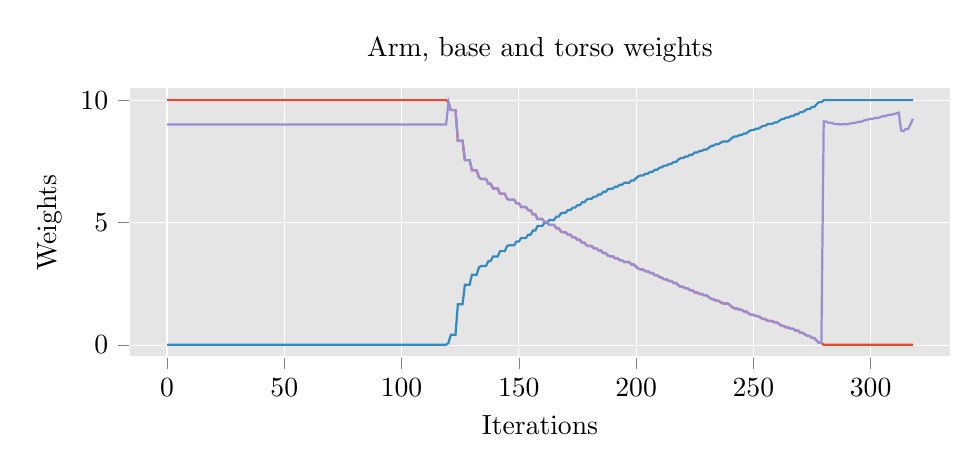
\begin{tikzpicture}

\definecolor{color1}{rgb}{0.203921568627451,0.541176470588235,0.741176470588235}
\definecolor{color0}{rgb}{0.886274509803922,0.290196078431373,0.2}
\definecolor{color2}{rgb}{0.596078431372549,0.556862745098039,0.835294117647059}

\begin{axis}[
title={Arm, base and torso weights},
xlabel={Iterations},
ylabel={Weights},
xmin=-15.9, xmax=333.9,
ymin=-0.4895, ymax=10.4995,
width=12cm,
height=5cm,
tick align=outside,
tick pos=left,
xmajorgrids,
x grid style={white},
ymajorgrids,
y grid style={white},
axis line style={white},
axis background/.style={fill=white!89.803921568627459!black}
]
\addplot [thick, color0, forget plot]
table {%
0 10
1 10
2 10
3 10
4 10
5 10
6 10
7 10
8 10
9 10
10 10
11 10
12 10
13 10
14 10
15 10
16 10
17 10
18 10
19 10
20 10
21 10
22 10
23 10
24 10
25 10
26 10
27 10
28 10
29 10
30 10
31 10
32 10
33 10
34 10
35 10
36 10
37 10
38 10
39 10
40 10
41 10
42 10
43 10
44 10
45 10
46 10
47 10
48 10
49 10
50 10
51 10
52 10
53 10
54 10
55 10
56 10
57 10
58 10
59 10
60 10
61 10
62 10
63 10
64 10
65 10
66 10
67 10
68 10
69 10
70 10
71 10
72 10
73 10
74 10
75 10
76 10
77 10
78 10
79 10
80 10
81 10
82 10
83 10
84 10
85 10
86 10
87 10
88 10
89 10
90 10
91 10
92 10
93 10
94 10
95 10
96 10
97 10
98 10
99 10
100 10
101 10
102 10
103 10
104 10
105 10
106 10
107 10
108 10
109 10
110 10
111 10
112 10
113 10
114 10
115 10
116 10
117 10
118 10
119 10
120 9.92348310154791
121 9.59048310165077
122 9.59048310165077
123 9.59048310165077
124 8.34166323466883
125 8.34166323466883
126 8.34166323466883
127 7.55051808763169
128 7.55051808763169
129 7.55051808763169
130 7.13813001521481
131 7.13813001521481
132 7.13813001521481
133 6.8366502472161
134 6.782214963872
135 6.782214963872
136 6.782214963872
137 6.58145710910527
138 6.58145710910527
139 6.39319805355104
140 6.39319805355104
141 6.39319805355104
142 6.17504402151094
143 6.17504402151094
144 6.17504402151094
145 5.97046383950916
146 5.93121961341934
147 5.93121961341934
148 5.93121961341934
149 5.78452381085447
150 5.78452381085447
151 5.64022767550553
152 5.64022767550553
153 5.64022767550553
154 5.50336072984546
155 5.50336072984546
156 5.33586637129325
157 5.33586637129325
158 5.14408439206331
159 5.14408439206331
160 5.14408439206331
161 5.02248826013462
162 5.02248826013462
163 4.90646639783278
164 4.90646639783278
165 4.90646639783278
166 4.76660352535582
167 4.76660352535582
168 4.63122664349342
169 4.60473511441951
170 4.60473511441951
171 4.50056263412593
172 4.50056263412593
173 4.3988678362718
174 4.3988678362718
175 4.29979616531319
176 4.29979616531319
177 4.17962749436673
178 4.17962749436673
179 4.06314733736329
180 4.04025968598617
181 4.04025968598617
182 3.95072887914645
183 3.95072887914645
184 3.86266957852752
185 3.86266957852752
186 3.7543569051649
187 3.7543569051649
188 3.64836952277614
189 3.6276861964953
190 3.6276861964953
191 3.54596055029517
192 3.54596055029517
193 3.46562973021897
194 3.46562973021897
195 3.38679573635182
196 3.38679573635182
197 3.38679573635182
198 3.29072433523839
199 3.29072433523839
200 3.19569371980191
201 3.12128891030488
202 3.08447625993113
203 3.08447625993113
204 3.01221354924889
205 3.01221354924889
206 2.94124678410257
207 2.94124678410257
208 2.85375935745956
209 2.85375935745956
210 2.76822084946326
211 2.7513031694567
212 2.68423114157031
213 2.68423114157031
214 2.61821389803748
215 2.61821389803748
216 2.53697320659966
217 2.53697320659966
218 2.44079202769906
219 2.37736934670253
220 2.37736934670253
221 2.31500562700777
222 2.31500562700777
223 2.23846101201079
224 2.23846101201079
225 2.14787925385901
226 2.14787925385901
227 2.08815201657904
228 2.08815201657904
229 2.02912813883255
230 2.02912813883255
231 1.95609268960976
232 1.88376684995326
233 1.86930765463614
234 1.8122507808957
235 1.8122507808957
236 1.75570919209946
237 1.6996656000052
238 1.6996656000052
239 1.6996656000052
240 1.6302055991507
241 1.54735225877438
242 1.49226111774091
243 1.49226111774091
244 1.43781740341127
245 1.43781740341127
246 1.37016889795776
247 1.37016889795776
248 1.28933407849659
249 1.23559180524832
250 1.23559180524832
251 1.18193683100528
252 1.18193683100528
253 1.12829596101549
254 1.06122733738008
255 1.06122733738008
256 0.993889957853116
257 0.98038791620549
258 0.98038791620549
259 0.926196289651467
260 0.926196289651467
261 0.858143189870261
262 0.789579424306385
263 0.77567688218032
264 0.719590924738094
265 0.719590924738094
266 0.662596057358317
267 0.662596057358317
268 0.589998650728475
269 0.589998650728475
270 0.500285020478426
271 0.500285020478426
272 0.439128346280988
273 0.374304974453691
274 0.374304974453691
275 0.287599501742187
276 0.287599501742187
277 0.173885935932702
278 0.0921676690621227
279 0.0921676690621227
280 0.01
281 0.01
282 0.01
283 0.01
284 0.01
285 0.01
286 0.01
287 0.01
288 0.01
289 0.01
290 0.01
291 0.01
292 0.01
293 0.01
294 0.01
295 0.01
296 0.01
297 0.01
298 0.01
299 0.01
300 0.01
301 0.01
302 0.01
303 0.01
304 0.01
305 0.01
306 0.01
307 0.01
308 0.01
309 0.01
310 0.01
311 0.01
312 0.01
313 0.01
314 0.01
315 0.01
316 0.01
317 0.01
318 0.01
};
\addplot [thick, color1, forget plot]
table {%
0 0.01
1 0.01
2 0.01
3 0.01
4 0.01
5 0.01
6 0.01
7 0.01
8 0.01
9 0.01
10 0.01
11 0.01
12 0.01
13 0.01
14 0.01
15 0.01
16 0.01
17 0.01
18 0.01
19 0.01
20 0.01
21 0.01
22 0.01
23 0.01
24 0.01
25 0.01
26 0.01
27 0.01
28 0.01
29 0.01
30 0.01
31 0.01
32 0.01
33 0.01
34 0.01
35 0.01
36 0.01
37 0.01
38 0.01
39 0.01
40 0.01
41 0.01
42 0.01
43 0.01
44 0.01
45 0.01
46 0.01
47 0.01
48 0.01
49 0.01
50 0.01
51 0.01
52 0.01
53 0.01
54 0.01
55 0.01
56 0.01
57 0.01
58 0.01
59 0.01
60 0.01
61 0.01
62 0.01
63 0.01
64 0.01
65 0.01
66 0.01
67 0.01
68 0.01
69 0.01
70 0.01
71 0.01
72 0.01
73 0.01
74 0.01
75 0.01
76 0.01
77 0.01
78 0.01
79 0.01
80 0.01
81 0.01
82 0.01
83 0.01
84 0.01
85 0.01
86 0.01
87 0.01
88 0.01
89 0.01
90 0.01
91 0.01
92 0.01
93 0.01
94 0.01
95 0.01
96 0.01
97 0.01
98 0.01
99 0.01
100 0.01
101 0.01
102 0.01
103 0.01
104 0.01
105 0.01
106 0.01
107 0.01
108 0.01
109 0.01
110 0.01
111 0.01
112 0.01
113 0.01
114 0.01
115 0.01
116 0.01
117 0.01
118 0.01
119 0.01
120 0.0865168984520928
121 0.419516898349228
122 0.419516898349228
123 0.419516898349228
124 1.66833676533117
125 1.66833676533117
126 1.66833676533117
127 2.45948191236831
128 2.45948191236831
129 2.45948191236831
130 2.87186998478519
131 2.87186998478519
132 2.87186998478519
133 3.1733497527839
134 3.227785036128
135 3.227785036128
136 3.227785036128
137 3.42854289089473
138 3.42854289089473
139 3.61680194644896
140 3.61680194644896
141 3.61680194644896
142 3.83495597848906
143 3.83495597848906
144 3.83495597848906
145 4.03953616049084
146 4.07878038658066
147 4.07878038658066
148 4.07878038658066
149 4.22547618914553
150 4.22547618914553
151 4.36977232449447
152 4.36977232449447
153 4.36977232449447
154 4.50663927015454
155 4.50663927015454
156 4.67413362870675
157 4.67413362870675
158 4.86591560793669
159 4.86591560793669
160 4.86591560793669
161 4.98751173986538
162 4.98751173986538
163 5.10353360216722
164 5.10353360216722
165 5.10353360216722
166 5.24339647464418
167 5.24339647464418
168 5.37877335650658
169 5.40526488558049
170 5.40526488558049
171 5.50943736587407
172 5.50943736587407
173 5.6111321637282
174 5.6111321637282
175 5.71020383468681
176 5.71020383468681
177 5.83037250563327
178 5.83037250563327
179 5.94685266263671
180 5.96974031401383
181 5.96974031401383
182 6.05927112085355
183 6.05927112085355
184 6.14733042147248
185 6.14733042147248
186 6.2556430948351
187 6.2556430948351
188 6.36163047722386
189 6.3823138035047
190 6.3823138035047
191 6.46403944970483
192 6.46403944970483
193 6.54437026978103
194 6.54437026978103
195 6.62320426364818
196 6.62320426364818
197 6.62320426364818
198 6.71927566476161
199 6.71927566476161
200 6.81430628019809
201 6.88871108969512
202 6.92552374006887
203 6.92552374006887
204 6.99778645075111
205 6.99778645075111
206 7.06875321589743
207 7.06875321589743
208 7.15624064254044
209 7.15624064254044
210 7.24177915053674
211 7.2586968305433
212 7.32576885842969
213 7.32576885842969
214 7.39178610196252
215 7.39178610196252
216 7.47302679340034
217 7.47302679340034
218 7.56920797230094
219 7.63263065329747
220 7.63263065329747
221 7.69499437299223
222 7.69499437299223
223 7.77153898798921
224 7.77153898798921
225 7.86212074614099
226 7.86212074614099
227 7.92184798342096
228 7.92184798342096
229 7.98087186116745
230 7.98087186116745
231 8.05390731039024
232 8.12623315004674
233 8.14069234536386
234 8.1977492191043
235 8.1977492191043
236 8.25429080790054
237 8.3103343999948
238 8.3103343999948
239 8.3103343999948
240 8.3797944008493
241 8.46264774122562
242 8.51773888225909
243 8.51773888225909
244 8.57218259658873
245 8.57218259658873
246 8.63983110204224
247 8.63983110204224
248 8.72066592150341
249 8.77440819475168
250 8.77440819475168
251 8.82806316899472
252 8.82806316899472
253 8.88170403898451
254 8.94877266261991
255 8.94877266261991
256 9.01611004214688
257 9.02961208379451
258 9.02961208379451
259 9.08380371034853
260 9.08380371034853
261 9.15185681012974
262 9.22042057569361
263 9.23432311781968
264 9.29040907526191
265 9.29040907526191
266 9.34740394264168
267 9.34740394264168
268 9.42000134927152
269 9.42000134927152
270 9.50971497952157
271 9.50971497952157
272 9.57087165371901
273 9.63569502554631
274 9.63569502554631
275 9.72240049825781
276 9.72240049825781
277 9.8361140640673
278 9.91783233093788
279 9.91783233093788
280 10
281 10
282 10
283 10
284 10
285 10
286 10
287 10
288 10
289 10
290 10
291 10
292 10
293 10
294 10
295 10
296 10
297 10
298 10
299 10
300 10
301 10
302 10
303 10
304 10
305 10
306 10
307 10
308 10
309 10
310 10
311 10
312 10
313 10
314 10
315 10
316 10
317 10
318 10
};
\addplot [thick, color2, forget plot]
table {%
0 9
1 9
2 9
3 9
4 9
5 9
6 9
7 9
8 9
9 9
10 9
11 9
12 9
13 9
14 9
15 9
16 9
17 9
18 9
19 9
20 9
21 9
22 9
23 9
24 9
25 9
26 9
27 9
28 9
29 9
30 9
31 9
32 9
33 9
34 9
35 9
36 9
37 9
38 9
39 9
40 9
41 9
42 9
43 9
44 9
45 9
46 9
47 9
48 9
49 9
50 9
51 9
52 9
53 9
54 9
55 9
56 9
57 9
58 9
59 9
60 9
61 9
62 9
63 9
64 9
65 9
66 9
67 9
68 9
69 9
70 9
71 9
72 9
73 9
74 9
75 9
76 9
77 9
78 9
79 9
80 9
81 9
82 9
83 9
84 9
85 9
86 9
87 9
88 9
89 9
90 9
91 9
92 9
93 9
94 9
95 9
96 9
97 9
98 9
99 9
100 9
101 9
102 9
103 9
104 9
105 9
106 9
107 9
108 9
109 9
110 9
111 9
112 9
113 9
114 9
115 9
116 9
117 9
118 9
119 9
120 9.92348310154791
121 9.59048310165077
122 9.59048310165077
123 9.59048310165077
124 8.34166323466883
125 8.34166323466883
126 8.34166323466883
127 7.55051808763169
128 7.55051808763169
129 7.55051808763169
130 7.13813001521481
131 7.13813001521481
132 7.13813001521481
133 6.8366502472161
134 6.782214963872
135 6.782214963872
136 6.782214963872
137 6.58145710910527
138 6.58145710910527
139 6.39319805355104
140 6.39319805355104
141 6.39319805355104
142 6.17504402151094
143 6.17504402151094
144 6.17504402151094
145 5.97046383950916
146 5.93121961341934
147 5.93121961341934
148 5.93121961341934
149 5.78452381085447
150 5.78452381085447
151 5.64022767550553
152 5.64022767550553
153 5.64022767550553
154 5.50336072984546
155 5.50336072984546
156 5.33586637129325
157 5.33586637129325
158 5.14408439206331
159 5.14408439206331
160 5.14408439206331
161 5.02248826013462
162 5.02248826013462
163 4.90646639783278
164 4.90646639783278
165 4.90646639783278
166 4.76660352535582
167 4.76660352535582
168 4.63122664349342
169 4.60473511441951
170 4.60473511441951
171 4.50056263412593
172 4.50056263412593
173 4.3988678362718
174 4.3988678362718
175 4.29979616531319
176 4.29979616531319
177 4.17962749436673
178 4.17962749436673
179 4.06314733736329
180 4.04025968598617
181 4.04025968598617
182 3.95072887914645
183 3.95072887914645
184 3.86266957852752
185 3.86266957852752
186 3.7543569051649
187 3.7543569051649
188 3.64836952277614
189 3.6276861964953
190 3.6276861964953
191 3.54596055029517
192 3.54596055029517
193 3.46562973021897
194 3.46562973021897
195 3.38679573635182
196 3.38679573635182
197 3.38679573635182
198 3.29072433523839
199 3.29072433523839
200 3.19569371980191
201 3.12128891030488
202 3.08447625993113
203 3.08447625993113
204 3.01221354924889
205 3.01221354924889
206 2.94124678410257
207 2.94124678410257
208 2.85375935745956
209 2.85375935745956
210 2.76822084946326
211 2.7513031694567
212 2.68423114157031
213 2.68423114157031
214 2.61821389803748
215 2.61821389803748
216 2.53697320659966
217 2.53697320659966
218 2.44079202769906
219 2.37736934670253
220 2.37736934670253
221 2.31500562700777
222 2.31500562700777
223 2.23846101201079
224 2.23846101201079
225 2.14787925385901
226 2.14787925385901
227 2.08815201657904
228 2.08815201657904
229 2.02912813883255
230 2.02912813883255
231 1.95609268960976
232 1.88376684995326
233 1.86930765463614
234 1.8122507808957
235 1.8122507808957
236 1.75570919209946
237 1.6996656000052
238 1.6996656000052
239 1.6996656000052
240 1.6302055991507
241 1.54735225877438
242 1.49226111774091
243 1.49226111774091
244 1.43781740341127
245 1.43781740341127
246 1.37016889795776
247 1.37016889795776
248 1.28933407849659
249 1.23559180524832
250 1.23559180524832
251 1.18193683100528
252 1.18193683100528
253 1.12829596101549
254 1.06122733738008
255 1.06122733738008
256 0.993889957853116
257 0.98038791620549
258 0.98038791620549
259 0.926196289651467
260 0.926196289651467
261 0.858143189870261
262 0.789579424306385
263 0.77567688218032
264 0.719590924738094
265 0.719590924738094
266 0.662596057358317
267 0.662596057358317
268 0.589998650728475
269 0.589998650728475
270 0.500285020478426
271 0.500285020478426
272 0.439128346280988
273 0.374304974453691
274 0.374304974453691
275 0.287599501742187
276 0.287599501742187
277 0.173885935932702
278 0.0921676690621227
279 0.0921676690621227
280 9.13000752298192
281 9.13000752298192
282 9.07237450595831
283 9.07237450595831
284 9.04843527296749
285 9.01898411878975
286 9.01898411878975
287 9.00740410838419
288 9.01117752977122
289 9.01117752977122
290 9.01654428506374
291 9.03674669976672
292 9.05865829047813
293 9.06343135094474
294 9.08962294118003
295 9.11958766330537
296 9.11958766330537
297 9.15910845625168
298 9.19156067010309
299 9.20766142295853
300 9.23966755027417
301 9.23966755027417
302 9.27075452630964
303 9.27075452630964
304 9.30096312898646
305 9.33726485841394
306 9.33726485841394
307 9.37861873678268
308 9.40498075120876
309 9.40498075120876
310 9.42993350880437
311 9.45960093930591
312 9.48825376440111
313 8.75807891211769
314 8.73696857174652
315 8.82243969317927
316 8.82243969317927
317 9.01440828068395
318 9.23796945929482
};
\end{axis}

\end{tikzpicture} \\ \vspace{-10pt}
	% This file was created by matplotlib2tikz v0.6.13.
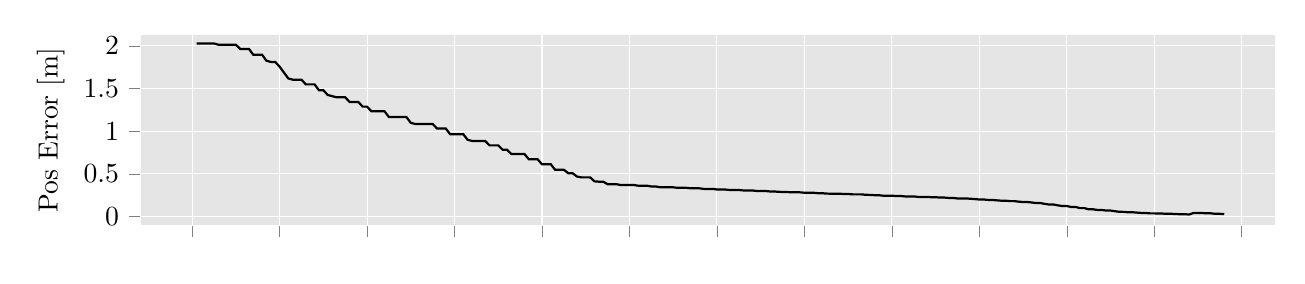
\begin{tikzpicture}

\begin{axis}[
%title={Position Error},
%xlabel={Iterations},
ylabel={Pos Error [m]},
xmin=-11.8, xmax=247.8,
ymin=-0.101362564657738, ymax=2.12861385781249,
width=16cm,
height=4cm,
tick align=outside,
tick pos=left,
xmajorgrids,
x grid style={white},
ymajorgrids,
y grid style={white},
axis line style={white},
axis background/.style={fill=white!89.803921568627459!black},
xticklabels=None
]
\addplot [thick, black, forget plot]
table {%
1 2.02725129315476
2 2.02725129315476
3 2.02725129315476
4 2.02725129315476
5 2.02725129315476
6 2.01303673676332
7 2.01303673676332
8 2.01303673676332
9 2.01303673676332
10 2.01303673676332
11 1.96300958682719
12 1.96300958682719
13 1.96300958682719
14 1.89434099367216
15 1.89434099367216
16 1.89434099367216
17 1.82513763722334
18 1.81128291499375
19 1.81128291499375
20 1.75578924578273
21 1.68652321113589
22 1.61737323470294
23 1.60356249494058
24 1.60356249494058
25 1.60356249494058
26 1.54836330471054
27 1.54836330471054
28 1.54836330471054
29 1.47950291486754
30 1.47950291486754
31 1.42454344147693
32 1.41082344518835
33 1.39711208163596
34 1.39711208163596
35 1.39711208163596
36 1.34235515959248
37 1.34235515959248
38 1.34235515959248
39 1.28775482652785
40 1.28775482652785
41 1.23333190750245
42 1.23333190750245
43 1.23333190750245
44 1.23333190750245
45 1.16559058578922
46 1.16559058578922
47 1.16559058578922
48 1.16559058578922
49 1.16559058578922
50 1.09822366971514
51 1.08480135971523
52 1.08480135971523
53 1.08480135971523
54 1.08480135971523
55 1.08480135971523
56 1.03130453105721
57 1.03130453105721
58 1.03130453105721
59 0.964926340356518
60 0.964926340356518
61 0.964926340356518
62 0.964926340356518
63 0.89920890165968
64 0.886157666629075
65 0.886157666629075
66 0.886157666629075
67 0.886157666629075
68 0.834308369442776
69 0.834308369442776
70 0.834308369442776
71 0.783112699750679
72 0.783112699750679
73 0.732707680923063
74 0.732707680923063
75 0.732707680923063
76 0.732707680923063
77 0.671089904559642
78 0.671089904559642
79 0.671089904559642
80 0.612988544489552
81 0.612988544489552
82 0.612988544489552
83 0.548610991376072
84 0.548610991376072
85 0.548610991376072
86 0.50810777807421
87 0.50810777807421
88 0.469034096537832
89 0.459507755843527
90 0.459507755843527
91 0.459507755843527
92 0.413057687868727
93 0.409036630170108
94 0.409036630170108
95 0.379357571635345
96 0.379357571635345
97 0.379357571635345
98 0.370020621462463
99 0.370020621462463
100 0.370020621462463
101 0.370020621462463
102 0.361937000205073
103 0.361937000205073
104 0.361937000205073
105 0.352747358684295
106 0.352747358684295
107 0.344543634584335
108 0.342943085547193
109 0.342943085547193
110 0.342943085547193
111 0.336961009870537
112 0.336961009870537
113 0.336961009870537
114 0.331146452461974
115 0.331146452461974
116 0.331146452461974
117 0.324187346918651
118 0.324187346918651
119 0.324187346918651
120 0.31764478266401
121 0.316360706886857
122 0.316360706886857
123 0.311413202945808
124 0.311413202945808
125 0.311413202945808
126 0.306557342253783
127 0.306557342253783
128 0.306557342253783
129 0.300693094104852
130 0.300693094104852
131 0.300693094104852
132 0.294957747045517
133 0.294957747045517
134 0.290511917659175
135 0.288328335797402
136 0.288328335797402
137 0.28403956636896
138 0.28403956636896
139 0.28403956636896
140 0.279814847078045
141 0.279814847078045
142 0.279814847078045
143 0.274604984374083
144 0.274604984374083
145 0.26949189525858
146 0.268472487224112
147 0.268472487224112
148 0.268472487224112
149 0.264472937836574
150 0.264472937836574
151 0.260503429940092
152 0.260503429940092
153 0.260503429940092
154 0.255579463642359
155 0.254037114133529
156 0.250703681672143
157 0.250703681672143
158 0.244891764087795
159 0.244891764087795
160 0.244891764087795
161 0.241074927637306
162 0.241074927637306
163 0.236316934188015
164 0.236316934188015
165 0.236316934188015
166 0.23063127388631
167 0.23063127388631
168 0.23063127388631
169 0.226846152570352
170 0.226846152570352
171 0.223064600064258
172 0.223064600064258
173 0.218352085381299
174 0.218352085381299
175 0.212661142563277
176 0.212661142563277
177 0.212661142563277
178 0.208861270727262
179 0.205045129458133
180 0.20022371271494
181 0.20022371271494
182 0.195340208948568
183 0.194358694726806
184 0.190415775330001
185 0.186405852946729
186 0.186405852946729
187 0.181334097311542
188 0.181334097311542
189 0.175087542791538
190 0.170754657920884
191 0.170754657920884
192 0.165222183762441
193 0.158367193114556
194 0.158367193114556
195 0.14819520559629
196 0.141168388364873
197 0.141168388364873
198 0.131328062026579
199 0.123458865139538
200 0.123458865139538
201 0.112899721076479
202 0.112899721076479
203 0.0995058525598717
204 0.0995058525598717
205 0.0855624372191504
206 0.0855624372191504
207 0.0777580291749132
208 0.0777580291749132
209 0.0708882526354914
210 0.0708882526354914
211 0.0630459575722875
212 0.0564492801901491
213 0.055278664142956
214 0.0510473182468205
215 0.0510473182468205
216 0.0471452367813468
217 0.0427278236645158
218 0.0427278236645158
219 0.0379828556297447
220 0.0379828556297447
221 0.0351386992603134
222 0.0351386992603134
223 0.0325437036300104
224 0.0325437036300104
225 0.0301528350056206
226 0.0273996797108044
227 0.0273996797108044
228 0.0248543553544655
229 0.0431279958900805
230 0.0416990360670842
231 0.0416990360670842
232 0.0380965270015528
233 0.0380965270015528
234 0.032357394799383
235 0.032357394799383
236 0.0290367171012285
};
\end{axis}

\end{tikzpicture} \\ \vspace{-5pt}
	% This file was created by matplotlib2tikz v0.6.13.
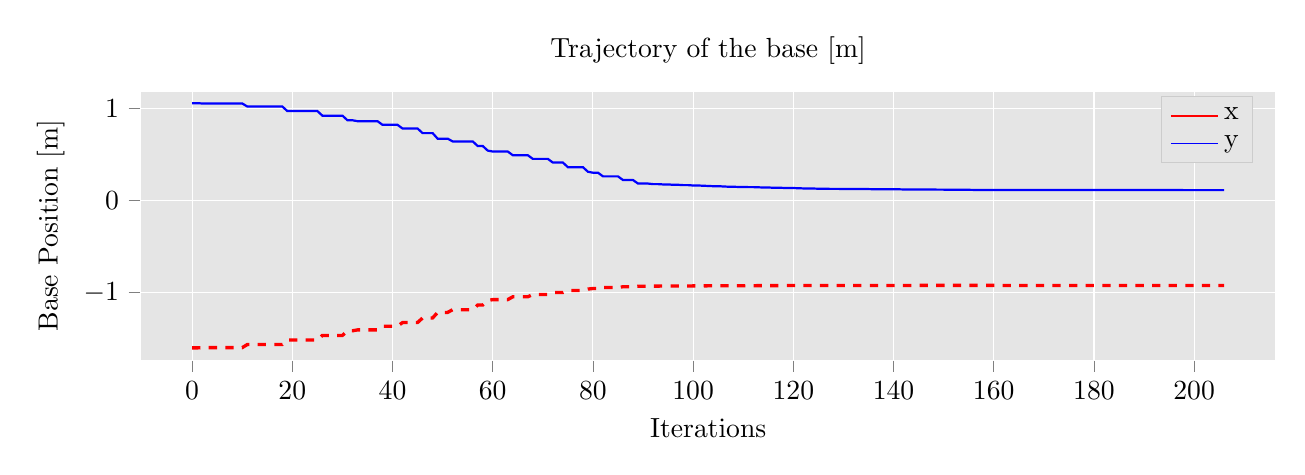
\begin{tikzpicture}

\begin{axis}[
title={Trajectory of the base [m]},
xlabel={Iterations},
ylabel={Base Position [m]},
xmin=-10.3, xmax=216.3,
ymin=-1.733, ymax=1.193,
width=16cm,
height=5cm,
tick align=outside,
tick pos=left,
xmajorgrids,
x grid style={white},
ymajorgrids,
y grid style={white},
axis line style={white},
axis background/.style={fill=white!89.803921568627459!black},
legend entries={{x},{y}},
legend cell align={left},
legend style={draw=white!80.0!black, fill=white!89.803921568627459!black}
]
\addlegendimage{no markers, red}
\addlegendimage{no markers, blue}
\addplot [very thick, red, dashed]
table {%
0 -1.6
1 -1.6
2 -1.597
3 -1.597
4 -1.597
5 -1.597
6 -1.597
7 -1.597
8 -1.597
9 -1.597
10 -1.597
11 -1.56405807907
12 -1.56405807907
13 -1.56405807907
14 -1.56405807907
15 -1.56405807907
16 -1.56405807907
17 -1.56405807907
18 -1.56405807907
19 -1.5144467024726
20 -1.5144467024726
21 -1.5144467024726
22 -1.5144467024726
23 -1.5144467024726
24 -1.5144467024726
25 -1.5144467024726
26 -1.46447406835882
27 -1.46447406835882
28 -1.46447406835882
29 -1.46447406835882
30 -1.46447406835882
31 -1.4144765073858
32 -1.4144765073858
33 -1.40447661782857
34 -1.40447661782857
35 -1.40447661782857
36 -1.40447661782857
37 -1.40447661782857
38 -1.36447675490682
39 -1.36447675490682
40 -1.36447675490682
41 -1.36447675490682
42 -1.32447679054794
43 -1.32447679054794
44 -1.32447679054794
45 -1.32447679054794
46 -1.27447680111136
47 -1.27447680111136
48 -1.27447680111136
49 -1.21447680390007
50 -1.21447680390007
51 -1.21447680390007
52 -1.18447680443961
53 -1.18447680443961
54 -1.18447680443961
55 -1.18447680443961
56 -1.18447680443961
57 -1.13447680474819
58 -1.13447680474819
59 -1.08447680480892
60 -1.07524046818883
61 -1.07524046818883
62 -1.07524046818883
63 -1.07524046818883
64 -1.04471312831992
65 -1.04471312831992
66 -1.04471312831992
67 -1.04471312831992
68 -1.01912016380541
69 -1.01912016380541
70 -1.01912016380541
71 -1.01912016380541
72 -0.997803032003999
73 -0.997803032003999
74 -0.997803032003999
75 -0.975218204865342
76 -0.975218204865342
77 -0.975218204865342
78 -0.975218204865342
79 -0.960820086794718
80 -0.95448140212623
81 -0.95448140212623
82 -0.943932479399614
83 -0.943932479399614
84 -0.943932479399614
85 -0.943932479399614
86 -0.935218731257354
87 -0.935218731257354
88 -0.935218731257354
89 -0.929284852778665
90 -0.929284852778665
91 -0.929284852778665
92 -0.928393962664367
93 -0.928393962664367
94 -0.92789253186454
95 -0.92789253186454
96 -0.927316291097345
97 -0.927316291097345
98 -0.926790137598026
99 -0.926790137598026
100 -0.92619691251295
101 -0.92619691251295
102 -0.925818433385451
103 -0.92546778223541
104 -0.925117196119697
105 -0.925117196119697
106 -0.924708749329195
107 -0.924331840806146
108 -0.924256471525831
109 -0.923981725990316
110 -0.923981725990316
111 -0.923721182188928
112 -0.923721182188928
113 -0.923471029182477
114 -0.923173563819612
115 -0.923173563819612
116 -0.922841503688237
117 -0.922841503688237
118 -0.922629596066127
119 -0.922629596066127
120 -0.922429901780819
121 -0.922198423028694
122 -0.921928330927893
123 -0.921928330927893
124 -0.921765795600105
125 -0.921583912581706
126 -0.921583912581706
127 -0.921421802577094
128 -0.921391632564588
129 -0.921391632564588
130 -0.921280607602169
131 -0.921280607602169
132 -0.921280607602169
133 -0.921179348118303
134 -0.921179348118303
135 -0.921179348118303
136 -0.921088020183272
137 -0.921088020183272
138 -0.921088020183272
139 -0.921088020183272
140 -0.92098782315279
141 -0.92098782315279
142 -0.920896038903192
143 -0.920896038903192
144 -0.920896038903192
145 -0.920828188741248
146 -0.92081601987693
147 -0.92081601987693
148 -0.92081601987693
149 -0.920779924680313
150 -0.920779924680313
151 -0.920742829785164
152 -0.920742829785164
153 -0.920729690565409
154 -0.920729690565409
155 -0.920729690565409
156 -0.920761689362019
157 -0.920771193755481
158 -0.920771193755481
159 -0.920804521650654
160 -0.920804521650654
161 -0.920833198421501
162 -0.920860653464771
163 -0.920860653464771
164 -0.920860653464771
165 -0.920891371061879
166 -0.920891371061879
167 -0.920923902603682
168 -0.920923902603682
169 -0.920943392149321
170 -0.920943392149321
171 -0.92096053619236
172 -0.92096053619236
173 -0.920979577191652
174 -0.920979577191652
175 -0.920998525549947
176 -0.920998525549947
177 -0.921010377106558
178 -0.921010377106558
179 -0.921024241612754
180 -0.921024241612754
181 -0.921034928289232
182 -0.921034928289232
183 -0.921045543618131
184 -0.921045543618131
185 -0.921059149463161
186 -0.921059149463161
187 -0.92107602181262
188 -0.92107602181262
189 -0.92108809065224
190 -0.92108809065224
191 -0.921103952717054
192 -0.92112076225457
193 -0.921134991614446
194 -0.921142511747214
195 -0.921158322304179
196 -0.921175014141524
197 -0.921175014141524
198 -0.921197055665799
199 -0.921220461611839
200 -0.921220461611839
201 -0.921250239732304
202 -0.921271735977755
203 -0.921271735977755
204 -0.921293916276054
205 -0.921293916276054
206 -0.92131691609802
};
\addplot [thick, blue]
table {%
0 1.06
1 1.06
2 1.057
3 1.057
4 1.057
5 1.057
6 1.057
7 1.057
8 1.057
9 1.057
10 1.057
11 1.02405807907
12 1.02405807907
13 1.02405807907
14 1.02405807907
15 1.02405807907
16 1.02405807907
17 1.02405807907
18 1.02405807907
19 0.974446702472604
20 0.974446702472604
21 0.974446702472604
22 0.974446702472604
23 0.974446702472604
24 0.974446702472604
25 0.974446702472604
26 0.924474068358822
27 0.924474068358822
28 0.924474068358822
29 0.924474068358822
30 0.924474068358822
31 0.874476507385801
32 0.874476507385801
33 0.864476617828568
34 0.864476617828568
35 0.864476617828568
36 0.864476617828568
37 0.864476617828568
38 0.824476754906818
39 0.824476754906818
40 0.824476754906818
41 0.824476754906818
42 0.784476790547937
43 0.784476790547937
44 0.784476790547937
45 0.784476790547937
46 0.734476801111359
47 0.734476801111359
48 0.734476801111359
49 0.674476803900066
50 0.674476803900066
51 0.674476803900066
52 0.644476804439605
53 0.644476804439605
54 0.644476804439605
55 0.644476804439605
56 0.644476804439605
57 0.594476804748189
58 0.594476804748189
59 0.544476804808915
60 0.534476804816172
61 0.534476804816172
62 0.534476804816172
63 0.534476804816172
64 0.494476804836641
65 0.494476804836641
66 0.494476804836641
67 0.494476804836641
68 0.454476804857484
69 0.454476804857484
70 0.454476804857484
71 0.454476804857484
72 0.414476804878707
73 0.414476804878707
74 0.414476804878707
75 0.364476804905702
76 0.364476804905702
77 0.364476804905702
78 0.364476804905702
79 0.314476804933276
80 0.304476804938844
81 0.304476804938844
82 0.264476804961333
83 0.264476804961333
84 0.264476804961333
85 0.264476804961333
86 0.224476804984123
87 0.224476804984123
88 0.224476804984123
89 0.186076091376362
90 0.186076091376362
91 0.186076091376362
92 0.180144792083999
93 0.180144792083999
94 0.176782658562525
95 0.176782658562525
96 0.172888030631495
97 0.172888030631495
98 0.169295215840986
99 0.169295215840986
100 0.165210350726714
101 0.165210350726714
102 0.162587334639323
103 0.160128842622251
104 0.157670209058382
105 0.157670209058382
106 0.154770852098351
107 0.152055300242471
108 0.151512161360925
109 0.149493372647414
110 0.149493372647414
111 0.147555332842583
112 0.147555332842583
113 0.145675781981009
114 0.143410690957842
115 0.143410690957842
116 0.140830220801471
117 0.140830220801471
118 0.139161694028975
119 0.139161694028975
120 0.137559121567055
121 0.135653665403669
122 0.133407502197722
123 0.133407502197722
124 0.132001695978516
125 0.130351715971188
126 0.130351715971188
127 0.128771189955413
128 0.128464747123751
129 0.128464747123751
130 0.127283583969367
131 0.127283583969367
132 0.127283583969367
133 0.12614633937926
134 0.12614633937926
135 0.12614633937926
136 0.125052376393463
137 0.125052376393463
138 0.125052376393463
139 0.125052376393463
140 0.123743992092906
141 0.123743992092906
142 0.122470318542358
143 0.122470318542358
144 0.122470318542358
145 0.121291588456311
146 0.121061295617525
147 0.121061295617525
148 0.121061295617525
149 0.12018636887809
150 0.12018636887809
151 0.119121956420319
152 0.119121956420319
153 0.1181404746572
154 0.1181404746572
155 0.1181404746572
156 0.117313694241853
157 0.11715914169192
158 0.11715914169192
159 0.116763204935963
160 0.116763204935963
161 0.116592045510715
162 0.116433945836664
163 0.116433945836664
164 0.116433945836664
165 0.116260975382485
166 0.116260975382485
167 0.116077146910816
168 0.116077146910816
169 0.115966222373377
170 0.115966222373377
171 0.115867466731942
172 0.115867466731942
173 0.115756349430836
174 0.115756349430836
175 0.115646319448912
176 0.115646319448912
177 0.115578836236855
178 0.115578836236855
179 0.115503951365173
180 0.115503951365173
181 0.115453038033154
182 0.115453038033154
183 0.115405960546106
184 0.115405960546106
185 0.115354700159115
186 0.115354700159115
187 0.115299834971672
188 0.115299834971672
189 0.115269252464994
190 0.115269252464994
191 0.115235496241995
192 0.11520560932771
193 0.115184312534541
194 0.115174886776325
195 0.115158178105164
196 0.115143686675652
197 0.115143686675652
198 0.115128066328859
199 0.115114972584817
200 0.115114972584817
201 0.115101937531827
202 0.115095571494139
203 0.115095571494139
204 0.115090080965047
205 0.115090080965047
206 0.115085504735328
};
\end{axis}

\end{tikzpicture} \vspace{-8pt}
	% This file was created by matplotlib2tikz v0.6.13.
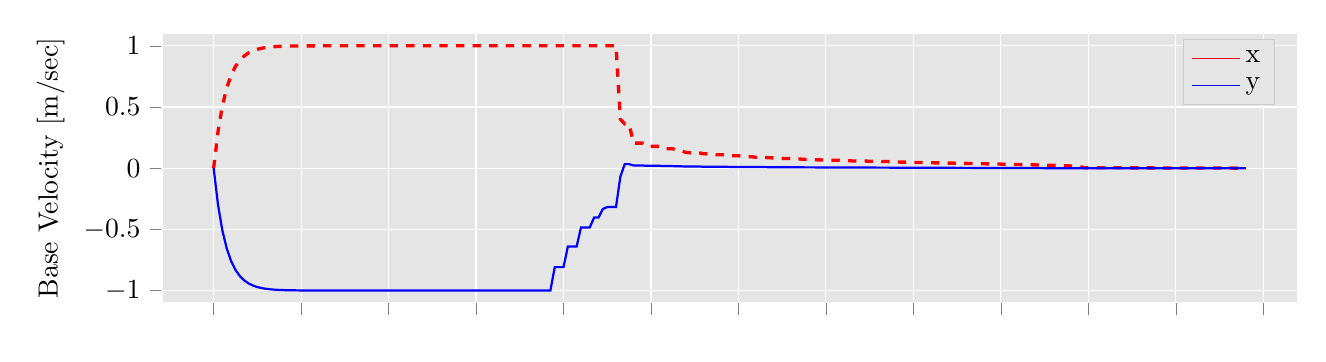
\begin{tikzpicture}

\begin{axis}[
%title={Velocity of the base},
%xlabel={Iterations},
ylabel={Base Velocity [m/sec]},
xmin=-11.8, xmax=247.8,
ymin=-1.09999999942715, ymax=1.09999999981315,
width=16cm,
height=5cm,
tick align=outside,
tick pos=left,
xmajorgrids,
x grid style={white},
ymajorgrids,
y grid style={white},
axis line style={white},
axis background/.style={fill=white!89.803921568627459!black},
legend entries={{x},{y}},
legend cell align={left},
legend style={draw=white!80.0!black, fill=white!89.803921568627459!black},
xticklabels=None
]
\addlegendimage{no markers, red}
\addlegendimage{no markers, blue}
\addplot [very thick, red, dashed]
table {%
0 0
1 0.3
2 0.51
3 0.657
4 0.7599
5 0.83193
6 0.882351
7 0.9176457
8 0.94235199
9 0.959646393
10 0.9717524751
11 0.98022673257
12 0.986158712799
13 0.9903110989593
14 0.99321776927151
15 0.995252438490057
16 0.99667670694304
17 0.997673694860128
18 0.998371586402089
19 0.998860110481463
20 0.999202077337024
21 0.999441454135916
22 0.999609017895142
23 0.999726312526599
24 0.999808418768619
25 0.999865893138033
26 0.999906125196623
27 0.999934287637636
28 0.999954001346345
29 0.999967800942442
30 0.999977460659709
31 0.999984222461796
32 0.999988955723257
33 0.99999226900628
34 0.999994588304396
35 0.999996211813077
36 0.999997348269154
37 0.999998143788408
38 0.999998700651885
39 0.99999909045632
40 0.999999363319424
41 0.999999554323597
42 0.999999688026518
43 0.999999781618562
44 0.999999847132993
45 0.999999892993095
46 0.999999925095167
47 0.999999947566617
48 0.999999963296632
49 0.999999974307642
50 0.99999998201535
51 0.999999987410745
52 0.999999991187521
53 0.999999993831265
54 0.999999995681885
55 0.99999999697732
56 0.999999997884124
57 0.999999998518887
58 0.99999999896322
59 0.999999999274254
60 0.999999999266646
61 0.999999999260229
62 0.999999999254642
63 0.99999999924963
64 0.999999999245016
65 0.999999999240674
66 0.999999999236518
67 0.999999999232486
68 0.999999999228536
69 0.999999999224638
70 0.99999999922077
71 0.999999999216919
72 0.999999999451843
73 0.999999999449151
74 0.999999999614406
75 0.999999999730084
76 0.999999999811059
77 0.999999999653793
78 0.999999999757655
79 0.999999999830358
80 0.999999999689156
81 0.999999999782409
82 0.999999999847687
83 0.999999999720907
84 0.999999999804635
85 0.999999999642022
86 0.999999999749416
87 0.999999999824591
88 0.999999999678588
89 0.999999999775012
90 0.999999999842508
91 0.999999999711419
92 0.999999999797994
93 0.399999999858596
94 0.361825896798878
95 0.361823368354502
96 0.204590163146216
97 0.204589747116436
98 0.204589539101547
99 0.178048936782746
100 0.178048889418124
101 0.178048865735812
102 0.178048853894657
103 0.159185751283843
104 0.159185748532558
105 0.159185747156915
106 0.141164637108274
107 0.141164636789825
108 0.128316529850266
109 0.125165047742916
110 0.125165047706024
111 0.125165047687577
112 0.117445366711686
113 0.116765558587293
114 0.116765558585086
115 0.109924866973211
116 0.109263213147836
117 0.109263213147571
118 0.101808168814982
119 0.101165238343519
120 0.101165238345109
121 0.0948895150700762
122 0.0929703636184211
123 0.0929703636184211
124 0.0889395719137215
125 0.0883288108229804
126 0.0883288108229804
127 0.0846037824557068
128 0.0840075750749145
129 0.0840075750749145
130 0.0797712197154456
131 0.0791909207825058
132 0.0791909207825058
133 0.0753287666650265
134 0.074763026640627
135 0.0721569851343673
136 0.0701139926083597
137 0.0701139926083597
138 0.0678526518267938
139 0.0673097528138626
140 0.0673097528138626
141 0.0652147490632162
142 0.0646794900570312
143 0.0646794900570312
144 0.0621090302151286
145 0.0615826613212095
146 0.0592363727339171
147 0.0581512854690635
148 0.0581512854690635
149 0.0581512854690635
150 0.0566075891998888
151 0.0560953080674546
152 0.0546139815372385
153 0.0541052742737761
154 0.0541034449211653
155 0.0522322547607478
156 0.0517275136175665
157 0.0494800341451014
158 0.0494785607577578
159 0.0473685325327003
160 0.046865921264711
161 0.0468648964768129
162 0.0457989224236112
163 0.0452966219727232
164 0.0438987542372921
165 0.0433968554876292
166 0.0433958348182677
167 0.0417243592389548
168 0.0412228352638405
169 0.0412221261915607
170 0.0403253550221604
171 0.0398234241244907
172 0.0389707612960742
173 0.0384687933716583
174 0.0373997119533456
175 0.0368962762277812
176 0.0355364135484438
177 0.0350327372535687
178 0.0355360118672388
179 0.0338516910553133
180 0.0332054159422728
181 0.0312419238488757
182 0.0312416258829675
183 0.0303618557882949
184 0.0295633053093955
185 0.0290010202862823
186 0.0273897491413432
187 0.0273896309976644
188 0.0266783668470014
189 0.0261584384072553
190 0.0250637972545833
191 0.0234658106505768
192 0.0234658497949994
193 0.0226484356763827
194 0.0203161144213964
195 0.0203163342883771
196 0.0175078461944597
197 0.0150705200723729
198 0.0150707956180802
199 0.00393583689959245
200 0.00376000560961766
201 0.00376006509779174
202 0.00353485349801651
203 0.00353492497354558
204 0.00324813005707571
205 0.00324821246954889
206 0.00294022799976553
207 0.0029402795221809
208 0.00275538974925705
209 0.00275543933595708
210 0.00258286526905384
211 0.00258292428201405
212 0.00237786034550612
213 0.00218937739101922
214 0.00215378508545145
215 0.00201836702050559
216 0.00201840651919678
217 0.00188850284301193
218 0.00173454535874542
219 0.00173459998674073
220 0.00156081060062599
221 0.00156084448051297
222 0.00145182454636893
223 0.00145185715482368
224 0.00134877134454349
225 0.00134880304082581
226 0.00125109545123585
227 0.00113560508465064
228 0.00113564097411648
229 0.00102649438455204
230 0.000733840406360542
231 0.000652886130858227
232 0.000652918822976152
233 0.000585068278189783
234 0.000585105112317842
235 0.000529559055498362
236 0.000529582062733399
};
\addplot [thick, blue]
table {%
0 0
1 -0.3
2 -0.51
3 -0.657
4 -0.7599
5 -0.83193
6 -0.882351
7 -0.9176457
8 -0.94235199
9 -0.959646393
10 -0.9717524751
11 -0.98022673257
12 -0.986158712799
13 -0.9903110989593
14 -0.99321776927151
15 -0.995252438490057
16 -0.99667670694304
17 -0.997673694860128
18 -0.998371586402089
19 -0.998860110481463
20 -0.999202077337024
21 -0.999441454135916
22 -0.999609017895142
23 -0.999726312526599
24 -0.999808418768619
25 -0.999865893138033
26 -0.999906125196623
27 -0.999934287637636
28 -0.999954001346345
29 -0.999967800942442
30 -0.999977460659709
31 -0.999984222461796
32 -0.999988955723257
33 -0.99999226900628
34 -0.999994588304396
35 -0.999996211813077
36 -0.999997348269154
37 -0.999998143788408
38 -0.999998700651885
39 -0.99999909045632
40 -0.999999363319424
41 -0.999999554323597
42 -0.999999688026518
43 -0.999999781618562
44 -0.999999847132993
45 -0.999999892993095
46 -0.999999925095167
47 -0.999999947566617
48 -0.999999963296632
49 -0.999999974307642
50 -0.99999998201535
51 -0.999999987410745
52 -0.999999991187521
53 -0.999999993831265
54 -0.999999995681885
55 -0.99999999697732
56 -0.999999997884124
57 -0.999999998518887
58 -0.99999999896322
59 -0.999999999274254
60 -0.999999999270743
61 -0.999999999267214
62 -0.999999999263668
63 -0.999999999260105
64 -0.999999999256525
65 -0.999999999252927
66 -0.999999999249313
67 -0.99999999924568
68 -0.99999999924203
69 -0.999999999238363
70 -0.999999999234677
71 -0.999999999230974
72 -0.999999999461682
73 -0.999999999459077
74 -0.999139369339006
75 -0.999139369339006
76 -0.999139369339006
77 -0.99913936821003
78 -0.808728750787954
79 -0.808728750787954
80 -0.808728749892674
81 -0.640177703553272
82 -0.640177703553272
83 -0.640177702843522
84 -0.484772674300587
85 -0.48477267350149
86 -0.484772674300587
87 -0.403446456325908
88 -0.403446455660714
89 -0.333378001196732
90 -0.318008612384317
91 -0.318008611836382
92 -0.318008612384317
93 -0.0689255480079944
94 0.033123137394042
95 0.0331220285927945
96 0.0220136013952464
97 0.0220134176038845
98 0.0220133257082035
99 0.0190377439380494
100 0.0190377229503266
101 0.0190377124564652
102 0.0190377072095345
103 0.0168987684308133
104 0.0168987672080607
105 0.0168987665966844
106 0.0148452626033866
107 0.0148452624613083
108 0.0132498375336823
109 0.0130041691477119
110 0.0130041691311728
111 0.0130041691229033
112 0.0119883872957416
113 0.012024817572462
114 0.0120248175714693
115 0.0111146226280297
116 0.0111520021480862
117 0.0111520021479668
118 0.0101640787814059
119 0.0102026622922612
120 0.0102026622935395
121 0.00935189640776924
122 0.00924054884454539
123 0.00924054884454539
124 0.0086392815507926
125 0.00868575207985389
126 0.00868575207985389
127 0.00811480457021736
128 0.00817208320247045
129 0.00817208320247045
130 0.00752199938017295
131 0.00759255136350329
132 0.00759255136350329
133 0.00697937464160835
134 0.00706186089013996
135 0.00657946145234516
136 0.00648997331086665
137 0.00648997331086665
138 0.00603557841329791
139 0.00614137285293054
140 0.00614137285293054
141 0.00569784063075072
142 0.00581222879930985
143 0.00581222879930985
144 0.00530127281731849
145 0.00542591753865191
146 0.00493043208976678
147 0.00499739489791831
148 0.00499739489791831
149 0.00499739489791831
150 0.00458075674495488
151 0.00472470677076455
152 0.00431604101467906
153 0.00446483744998895
154 0.00446062325597755
155 0.00400200310299939
156 0.00415003010611961
157 0.0038523640040677
158 0.00384880051347668
159 0.00337125045267695
160 0.00352126047670399
161 0.003518693237045
162 0.00315173974578196
163 0.00330253029321702
164 0.0028880042398776
165 0.00303984390670854
166 0.0030371310499043
167 0.00258558789841342
168 0.00273885328538321
169 0.00273687720908373
170 0.00239180132369484
171 0.00254425540634951
172 0.00220247778443559
173 0.00235581609203322
174 0.00196332489460331
175 0.00211845513881316
176 0.00169090304180869
177 0.00185066286561906
178 0.00168951545150214
179 0.00167001211848221
180 0.00132934603088596
181 0.00128303079092762
182 0.00128169394056528
183 0.000899579893786159
184 0.00102712294088919
185 0.00068253040606397
186 0.000687492954586867
187 0.000686501951555275
188 0.000278978571675385
189 0.000457186262024756
190 1.41135635072463e-05
191 1.71669591025941e-05
192 1.64938256650374e-05
193 -0.000412070701711152
194 -0.000505484127313667
195 -0.000506213275343632
196 -0.000960961092610291
197 -0.00130867250885863
198 -0.00130894074304675
199 -0.000675613043893916
200 -0.000683929196060617
201 -0.000683964481650769
202 -0.00068691502785033
203 -0.000686955034995684
204 -0.00068598684136027
205 -0.000686033284726024
206 -0.000675701802064443
207 -0.000675731001415412
208 -0.000661751412379645
209 -0.000661779588324128
210 -0.000643184466468209
211 -0.000643218066990977
212 -0.000617644687648099
213 -0.000586331279009221
214 -0.00057940330262841
215 -0.000550080880721429
216 -0.000550103477460803
217 -0.000520155573095623
218 -0.000482443784180148
219 -0.000482475081193471
220 -0.000437487389922546
221 -0.00043750681378135
222 -0.000407951562535111
223 -0.000407970264448685
224 -0.000379040852601926
225 -0.000379059036805547
226 -0.000350992640100194
227 -0.000317207163783006
228 -0.000317227763595251
229 -0.000284917622939736
230 -0.000347691751702064
231 -0.000323534975975726
232 -0.000323553575192973
233 -0.000296967845389445
234 -0.000296988822111123
235 -0.000267725566757142
236 -0.000267738691484418
};
\end{axis}

\end{tikzpicture} \vspace{-5pt}
	% This file was created by matplotlib2tikz v0.6.13.
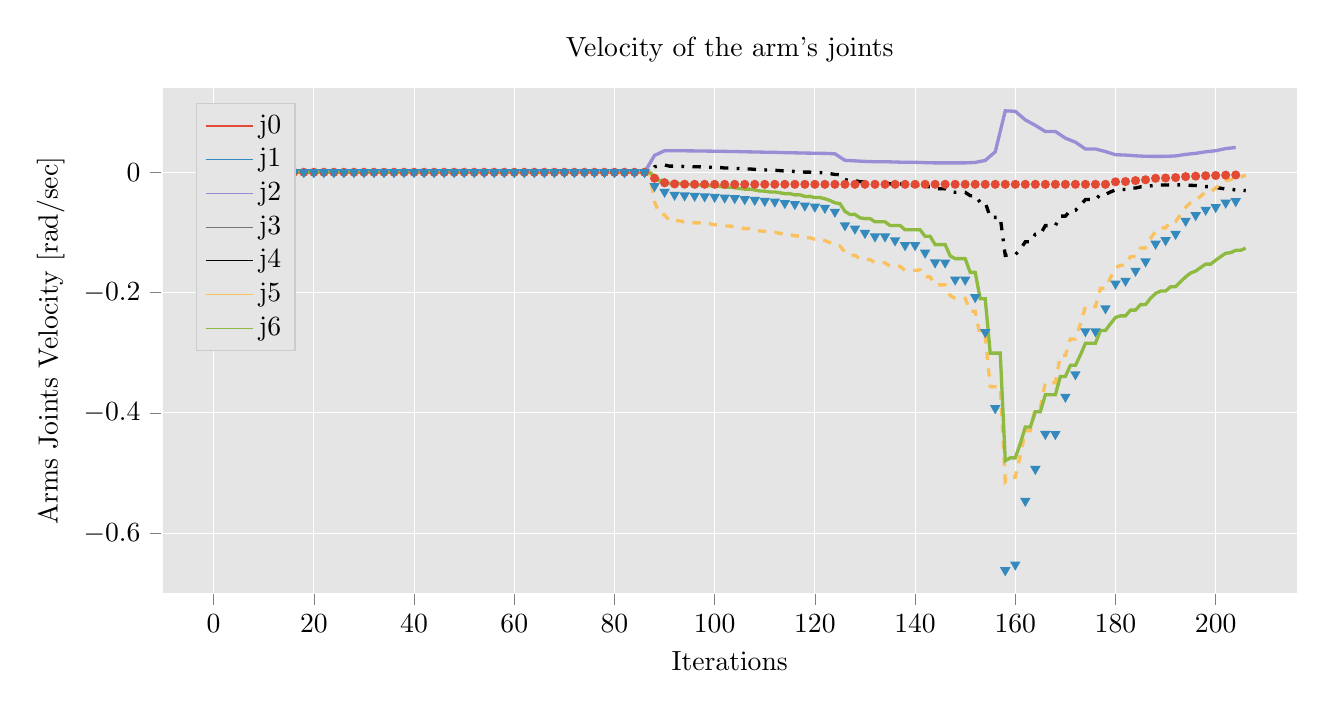
\begin{tikzpicture}

\definecolor{color1}{rgb}{0.203921568627451,0.541176470588235,0.741176470588235}
\definecolor{color0}{rgb}{0.886274509803922,0.290196078431373,0.2}
\definecolor{color3}{rgb}{0.984313725490196,0.756862745098039,0.368627450980392}
\definecolor{color2}{rgb}{0.596078431372549,0.556862745098039,0.835294117647059}
\definecolor{color4}{rgb}{0.556862745098039,0.729411764705882,0.258823529411765}

\begin{axis}[
title={Velocity of the arm's joints},
xlabel={Iterations},
ylabel={Arms Joints Velocity [rad/sec]},
xmin=-10.3, xmax=216.3,
ymin=-0.699705577747706, ymax=0.140284172952257,
width=16cm,
height=8cm,
tick align=outside,
tick pos=left,
xmajorgrids,
x grid style={white},
ymajorgrids,
y grid style={white},
axis line style={white},
axis background/.style={fill=white!89.803921568627459!black},
legend style={at={(0.03,0.97)}, anchor=north west, draw=white!80.0!black, fill=white!89.803921568627459!black},
legend entries={{j0},{j1},{j2},{j3},{j4},{j5},{j6}},
legend cell align={left}
]
\addlegendimage{no markers, color0}
\addlegendimage{no markers, color1}
\addlegendimage{no markers, color2}
\addlegendimage{no markers, lightgray!62.222222222222221!black}
\addlegendimage{no markers, black}
\addlegendimage{no markers, color3}
\addlegendimage{no markers, color4}
\addplot [very thick, color0, mark=*, mark size=1, mark options={solid}, only marks]
table {%
0 0
2 0
4 0
6 0
8 0
10 0
12 0
14 0
16 1.0842021724855e-19
18 0
20 -1.35525271560688e-20
22 0
24 0
26 0
28 0
30 0
32 0
34 0
36 0
38 0
40 0
42 0
44 0
46 -1.65436122510606e-24
48 8.27180612553028e-25
50 4.13590306276514e-25
52 0
54 1.03397576569128e-25
56 -5.16987882845642e-26
58 0
60 0
62 -5.28319920364145e-11
64 -5.33445211831421e-11
66 -5.38620402619483e-11
68 -5.43845493812534e-11
70 -5.49121470950348e-11
72 -5.54448661461981e-11
74 -5.59827393860693e-11
76 -5.65258652602055e-11
78 -5.70742437686067e-11
80 -5.76279406139246e-11
82 -5.81869886474851e-11
84 -5.87514534635195e-11
86 -5.93213680217738e-11
88 -0.0100000000298042
90 -0.017500000007451
92 -0.0193750000018628
94 -0.0198437500004657
96 -0.0199609375001164
98 -0.0199902343750291
100 -0.0199975585937573
102 -0.0199993896484393
104 -0.0199998474121098
106 -0.0199999618530275
108 -0.0199999904632569
110 -0.0199999976158142
112 -0.0199999994039536
114 -0.019999999999881
116 -0.02
118 -0.02
120 -0.02
122 -0.02
124 -0.02
126 -0.02
128 -0.02
130 -0.02
132 -0.02
134 -0.02
136 -0.02
138 -0.02
140 -0.02
142 -0.02
144 -0.02
146 -0.02
148 -0.02
150 -0.02
152 -0.02
154 -0.02
156 -0.02
158 -0.02
160 -0.02
162 -0.02
164 -0.02
166 -0.02
168 -0.02
170 -0.02
172 -0.02
174 -0.02
176 -0.02
178 -0.02
180 -0.0158740685618244
182 -0.0153931359500379
184 -0.0138026889917807
186 -0.0124211501456629
188 -0.0100015392202426
190 -0.0095518676683817
192 -0.00877233333082943
194 -0.00720196314277957
196 -0.00647678987375005
198 -0.0057331708971329
200 -0.00535355906508371
202 -0.00473967363927567
204 -0.00450972903305606
};
\addplot [very thick, color1, mark=triangle*, mark size=1, mark options={solid,rotate=180}, only marks]
table {%
0 0
2 -1.0842021724855e-19
4 -1.0842021724855e-19
6 -1.0842021724855e-19
8 -1.0842021724855e-19
10 -1.0842021724855e-19
12 0
14 0
16 0
18 -5.42101086242752e-20
20 -1.35525271560688e-20
22 0
24 -6.7762635780344e-21
26 -1.6940658945086e-21
28 -1.6940658945086e-21
30 0
32 -2.11758236813575e-22
34 -1.05879118406788e-22
36 -5.29395592033938e-23
38 0
40 -1.32348898008484e-23
42 -1.32348898008484e-23
44 -3.30872245021211e-24
46 0
48 0
50 -4.13590306276514e-25
52 -2.06795153138257e-25
54 -1.03397576569128e-25
56 0
58 0
60 0
62 -4.78369674601631e-11
64 -4.83010392749936e-11
66 -4.87696292855375e-11
68 -4.9242737600215e-11
70 -4.97204532320245e-11
72 -5.02028061049459e-11
74 -5.06898259261188e-11
76 -5.11816017085415e-11
78 -5.1678133452214e-11
80 -5.21794807882558e-11
82 -5.26856734238065e-11
84 -5.31967706647249e-11
86 -5.37128024349909e-11
88 -0.0229604650404843
90 -0.0326906703801806
92 -0.0375356702320031
94 -0.0385962227693658
96 -0.0392706316851977
98 -0.0401355767952046
100 -0.0410266861686532
102 -0.0421691156890109
104 -0.0430898539925271
106 -0.044763522267914
108 -0.0461059346700655
110 -0.0476653560572003
112 -0.0487925718060801
114 -0.0512158013456615
116 -0.0529999254301903
118 -0.0553956188193768
120 -0.0571917877196441
122 -0.0592600910055702
124 -0.0657415843790988
126 -0.0882624114274274
128 -0.0937430700957926
130 -0.100981329937883
132 -0.106700505590667
134 -0.106773795058327
136 -0.113388928992332
138 -0.121339160180093
140 -0.121339160180093
142 -0.133713735734453
144 -0.149990269990794
146 -0.150081570635811
148 -0.178496665734961
150 -0.178569746573562
152 -0.207647719727777
154 -0.265771505119499
156 -0.392192998800836
158 -0.661524225443162
160 -0.652060667814417
162 -0.546229016091103
164 -0.493183303974978
166 -0.435071505470748
168 -0.435180288667053
170 -0.373263201507692
172 -0.335842301117052
174 -0.264311308917872
176 -0.264401457804908
178 -0.226153986446429
180 -0.185197222261064
182 -0.180398833116305
184 -0.163793316777835
186 -0.14834994162116
188 -0.118844805476923
190 -0.11300968594613
192 -0.102653201779496
194 -0.0807387103170511
196 -0.0714316789680384
198 -0.0624739561296378
200 -0.0579078288626683
202 -0.0506302107886316
204 -0.0480615759420165
};
\addplot [very thick, color2]
table {%
0 0
2 0
4 -1.0842021724855e-19
6 -1.0842021724855e-19
8 -1.0842021724855e-19
10 -1.0842021724855e-19
12 -1.0842021724855e-19
14 0
16 -5.42101086242752e-20
18 -2.71050543121376e-20
20 0
22 -6.7762635780344e-21
24 -6.7762635780344e-21
26 -1.6940658945086e-21
28 -1.6940658945086e-21
30 -4.2351647362715e-22
32 -2.11758236813575e-22
34 -1.05879118406788e-22
36 -5.29395592033938e-23
38 0
40 -1.32348898008484e-23
42 -6.61744490042422e-24
44 -3.30872245021211e-24
46 -1.65436122510606e-24
48 -8.27180612553028e-25
50 0
52 -2.06795153138257e-25
54 -1.03397576569128e-25
56 -5.16987882845642e-26
58 -2.58493941422821e-26
60 0
62 -4.81251420008169e-11
64 -4.85920094309492e-11
66 -4.90634222702693e-11
68 -4.95393806271976e-11
70 -5.00199739484133e-11
72 -5.05052325915772e-11
74 -5.09951862638289e-11
76 -5.14899245202677e-11
78 -5.19894475777341e-11
80 -5.24938150673476e-11
82 -5.30030570215084e-11
84 -5.35172331797562e-11
86 -5.40363734660709e-11
88 0.0280327470747409
90 0.0358457672066788
92 0.0359129110943181
94 0.03567358649435
96 0.0355006555457565
98 0.0352709649948503
100 0.0350306763036447
102 0.0347233062789331
104 0.0345047520873177
106 0.0340484696931078
108 0.0337457009054476
110 0.0333756084722837
112 0.0331304519076355
114 0.0326313175597288
116 0.0323105574555889
118 0.0319254735619353
120 0.0316623846661011
122 0.0314023192678998
124 0.0307088351280693
126 0.0198536197666636
128 0.0189459292760229
130 0.0180790446666461
132 0.0175611061837919
134 0.0175592430139907
136 0.0170558935970478
138 0.0165759068875077
140 0.0165759068875077
142 0.016043458693033
144 0.0156012569881466
146 0.0155975700792514
148 0.0156177321613598
150 0.0156141134605933
152 0.0164079600754668
154 0.0196390220093228
156 0.0341155976773544
158 0.102102820647714
160 0.101355254107457
162 0.0870552352863174
164 0.0779827895736372
166 0.0677960772392341
168 0.0677789020892197
170 0.0567294812642832
172 0.0500290918840398
174 0.0387245169358087
176 0.038710283849164
178 0.0344315172033015
180 0.0291805039483196
182 0.0285965616974953
184 0.0273951315970479
186 0.0265705600098816
188 0.0263686334450229
190 0.0265039277915179
192 0.0271592939446448
194 0.0297163691651581
196 0.031413174945186
198 0.0340487414800164
200 0.0358295002745964
202 0.039434491680096
204 0.0411410923375538
};
\addplot [very thick, lightgray!62.222222222222221!black, mark=asterisk*, mark size=1, mark options={solid}, only marks]
table {%
0 0
2 -1.0842021724855e-19
4 -1.0842021724855e-19
6 -1.0842021724855e-19
8 -1.0842021724855e-19
10 -1.0842021724855e-19
12 -1.0842021724855e-19
14 -1.0842021724855e-19
16 -5.42101086242752e-20
18 -2.71050543121376e-20
20 -1.35525271560688e-20
22 -6.7762635780344e-21
24 -3.3881317890172e-21
26 -1.6940658945086e-21
28 -1.6940658945086e-21
30 -4.2351647362715e-22
32 -2.11758236813575e-22
34 0
36 0
38 -5.29395592033938e-23
40 -1.32348898008484e-23
42 0
44 0
46 -1.65436122510606e-24
48 -8.27180612553028e-25
50 -4.13590306276514e-25
52 -4.13590306276514e-25
54 -1.03397576569128e-25
56 0
58 0
60 0
62 -4.84133164330505e-11
64 -4.88829794784845e-11
66 -4.9357215146581e-11
68 -4.98360235457601e-11
70 -5.03194947732225e-11
72 -5.08076590782086e-11
74 -5.13005467099592e-11
76 -5.17982475488343e-11
78 -5.2300761594834e-11
80 -5.28081493464394e-11
82 -5.33204405107901e-11
84 -5.38376955863673e-11
86 -5.4359944497151e-11
88 -0.0179938779746514
90 -0.0174540616343219
92 -0.0174540616343219
94 -0.0164068179362631
96 -0.0157296003448519
98 -0.0149228037998674
100 -0.0141605276789742
102 -0.0133032732570268
104 -0.0122304388522445
106 -0.0117145290261988
108 -0.0105396229037189
110 -0.0100091273998246
112 -0.0096045686813202
114 -0.00920824917640015
116 -0.00874387351050332
118 -0.00820995358655319
120 -0.00787087704461209
122 -0.00716228960364917
124 -0.00672084137961626
126 -0.0061213423285551
128 -0.00581196855816923
130 -0.00575384887258767
132 -0.00552311372082803
134 -0.00530218917199532
136 -0.00530218917199532
138 -0.00508789235962759
140 -0.00508789235962759
142 -0.00483135477352192
144 -0.00458209090726181
146 -0.00435049372323526
148 -0.00430467281416247
150 -0.00413202769250542
152 -0.00392024695423077
154 -0.00371788118437166
156 -0.00371788118437167
158 -0.00349278465561031
160 -0.00335045051598026
162 -0.00321216247115297
164 -0.00308229309185837
166 -0.00292558104967888
168 -0.00274847906627595
170 -0.00263853990362417
172 -0.00253189891585226
174 -0.00240317115030386
176 -0.00225640632597468
178 -0.00216615007293619
180 -0.00205603744422822
182 -0.00197336271644488
184 -0.00189277471323201
186 -0.00179652421750642
188 -0.00168680775454089
190 -0.00161714111509959
192 -0.0015341940601612
194 -0.00139680871297188
196 0.0011095984712565
198 0.00496956132317292
200 0.0069212461441987
202 0.00996574969876916
204 0.0109708120461363
};
\addplot [very thick, black, dash pattern=on 1pt off 3pt on 3pt off 3pt]
table {%
0 0
1 0
2 0
3 0
4 0
5 -1.0842021724855e-19
6 -1.0842021724855e-19
7 0
8 0
9 0
10 -1.0842021724855e-19
11 -1.0842021724855e-19
12 -1.0842021724855e-19
13 -1.0842021724855e-19
14 -1.0842021724855e-19
15 -1.0842021724855e-19
16 -1.0842021724855e-19
17 0
18 -2.71050543121376e-20
19 -2.71050543121376e-20
20 0
21 0
22 -6.7762635780344e-21
23 -6.7762635780344e-21
24 -3.3881317890172e-21
25 -3.3881317890172e-21
26 -3.3881317890172e-21
27 -1.6940658945086e-21
28 0
29 0
30 -4.2351647362715e-22
31 0
32 -2.11758236813575e-22
33 -2.11758236813575e-22
34 -1.05879118406788e-22
35 -1.05879118406788e-22
36 -5.29395592033938e-23
37 -5.29395592033938e-23
38 -2.64697796016969e-23
39 0
40 -1.32348898008484e-23
41 0
42 0
43 -6.61744490042422e-24
44 -3.30872245021211e-24
45 -1.65436122510606e-24
46 0
47 -8.27180612553028e-25
48 0
49 -8.27180612553028e-25
50 0
51 -2.06795153138257e-25
52 -2.06795153138257e-25
53 -2.06795153138257e-25
54 -1.03397576569128e-25
55 0
56 -5.16987882845642e-26
57 0
58 0
59 -1.29246970711411e-26
60 -1.29246970711411e-26
61 -4.84669562513321e-11
62 -4.87014909737044e-11
63 -4.89371453516602e-11
64 -4.91739496344401e-11
65 -4.94119038220442e-11
66 -4.96510081313128e-11
67 -4.98912623454056e-11
68 -5.01326665727428e-11
69 -5.03752509541447e-11
70 -5.06190157064518e-11
71 -5.08639606128236e-11
72 -5.11100857816804e-11
73 -5.13573912130222e-11
74 -5.16059070476693e-11
75 -5.1855633394042e-11
76 -5.21065703605605e-11
77 -5.23587178388046e-11
78 -5.26120757203541e-11
79 -5.28666743628697e-11
80 -5.3122483517111e-11
81 -5.33795334323184e-11
82 -5.36378240000718e-11
83 -5.38973555456318e-11
84 -5.41581581013986e-11
85 -5.44202014181316e-11
86 -5.46835157450715e-11
87 -5.49481009737979e-11
88 0.00907756171617541
89 0.0110331793033056
90 0.0120489514693584
91 0.0101819236571973
92 0.0101963724331739
93 0.0101954103317678
94 0.00951057654999714
95 0.00950691728499617
96 0.00905564977414641
97 0.00904931905321964
98 0.0084748201254057
99 0.00846826269894548
100 0.00788260583782679
101 0.00787484476345712
102 0.0071413020937256
103 0.00713617548313066
104 0.00661863158707836
105 0.00609559997400068
106 0.00554641667715483
107 0.00554017767589826
108 0.0048307138914727
109 0.00410851732265348
110 0.00395296958279546
111 0.00336115027490611
112 0.00335644897493095
113 0.00274320255815933
114 0.00211204164008328
115 0.00210630315561576
116 0.00128398190421899
117 0.00127711882639514
118 0.00024292502316675
119 0.000238350859761121
120 -0.000493317241580193
121 -0.000497754548073487
122 -0.00126304921394299
123 -0.00225926870929321
124 -0.00356182728970286
125 -0.00398571077798088
126 -0.0121982360989544
127 -0.013912608494494
128 -0.0139179604118773
129 -0.0156586947628947
130 -0.0160204439373475
131 -0.0160246769255898
132 -0.0175476725395176
133 -0.0175476725395176
134 -0.0175518943155304
135 -0.0192445570721777
136 -0.0192445570721777
137 -0.0192488297197494
138 -0.0211610568751506
139 -0.0211610568751506
140 -0.0211610568751506
141 -0.020932006947376
142 -0.0239801479404097
143 -0.0239856558730766
144 -0.0275004816650143
145 -0.0275004816650143
146 -0.027505926388984
147 -0.0321459593586042
148 -0.0332735082503915
149 -0.0332735082503916
150 -0.033277910976603
151 -0.0388973183884716
152 -0.0389030485313349
153 -0.0500145801249874
154 -0.0500204847664704
155 -0.0749405626103001
156 -0.0749405626103
157 -0.0749464188742449
158 -0.138130898493836
159 -0.136870602682766
160 -0.136874691930295
161 -0.12830332000693
162 -0.115594472305352
163 -0.115598203441393
164 -0.102987941674595
165 -0.102992443998021
166 -0.0886665432257567
167 -0.0886665432257568
168 -0.0886716313504316
169 -0.0729340507144971
170 -0.0729372092571373
171 -0.0632496802724416
172 -0.0632527440588025
173 -0.0547588575804294
174 -0.045363637116093
175 -0.0453636371160931
176 -0.0453678536568099
177 -0.0367977173613572
178 -0.0368003104157055
179 -0.0326584640398517
180 -0.0293811813310156
181 -0.0285294715414068
182 -0.0285315237158573
183 -0.026203304300218
184 -0.0262053158582742
185 -0.0242482793620052
186 -0.024250693484366
187 -0.0225859041122879
188 -0.0215986531590014
189 -0.0212172786606541
190 -0.0212190435207714
191 -0.0208879196216149
192 -0.020890026597789
193 -0.0208900746643763
194 -0.0212046492757298
195 -0.0216849405869357
196 -0.0220250587899677
197 -0.0228465908455734
198 -0.0238046664138047
199 -0.0238046664138047
200 -0.0251259473953038
201 -0.0265392488674483
202 -0.0279895234809487
203 -0.0282794302226522
204 -0.029426883959957
205 -0.029426883959957
206 -0.0305564278661351
};
\addplot [very thick, color3, dashed]
table {%
0 0
1 -3.46944695195361e-18
2 -1.0842021724855e-19
3 -1.0842021724855e-19
4 -1.0842021724855e-19
5 -1.0842021724855e-19
6 -1.0842021724855e-19
7 -1.0842021724855e-19
8 -1.0842021724855e-19
9 -1.0842021724855e-19
10 -1.0842021724855e-19
11 -2.16840434497101e-19
12 0
13 -1.0842021724855e-19
14 -1.0842021724855e-19
15 -1.0842021724855e-19
16 -5.42101086242752e-20
17 -5.42101086242752e-20
18 -2.71050543121376e-20
19 -2.71050543121376e-20
20 -1.35525271560688e-20
21 -1.35525271560688e-20
22 -6.7762635780344e-21
23 -6.7762635780344e-21
24 -3.3881317890172e-21
25 -3.3881317890172e-21
26 -3.3881317890172e-21
27 0
28 -8.470329472543e-22
29 -8.470329472543e-22
30 -4.2351647362715e-22
31 -4.2351647362715e-22
32 -2.11758236813575e-22
33 -2.11758236813575e-22
34 -1.05879118406788e-22
35 -1.05879118406788e-22
36 -5.29395592033938e-23
37 -5.29395592033938e-23
38 -2.64697796016969e-23
39 -2.64697796016969e-23
40 -2.64697796016969e-23
41 0
42 -6.61744490042422e-24
43 0
44 -3.30872245021211e-24
45 -1.65436122510606e-24
46 0
47 -8.27180612553028e-25
48 -8.27180612553028e-25
49 -4.13590306276514e-25
50 -4.13590306276514e-25
51 -2.06795153138257e-25
52 0
53 -2.06795153138257e-25
54 -1.03397576569128e-25
55 0
56 0
57 -2.58493941422821e-26
58 -2.58493941422821e-26
59 0
60 0
61 -4.87537431216253e-11
62 -4.89896655143582e-11
63 -4.92267141763078e-11
64 -4.94649196819755e-11
65 -4.9704281922941e-11
66 -4.99448010076245e-11
67 -5.01864768276059e-11
68 -5.04293094913053e-11
69 -5.06733292479633e-11
70 -5.09185364228407e-11
71 -5.11649307990969e-11
72 -5.14125122683118e-11
73 -5.16612810473258e-11
74 -5.19112674937997e-11
75 -5.21624714993132e-11
76 -5.2414893280707e-11
77 -5.26685326211404e-11
78 -5.29233896290338e-11
79 -5.31794947704681e-11
80 -5.34368176877825e-11
81 -5.36953887386379e-11
82 -5.39552077061939e-11
83 -5.4216274915711e-11
84 -5.44786206164299e-11
85 -5.47422144506898e-11
86 -5.50070867761515e-11
87 -5.52732377012352e-11
88 -0.0496341876054172
89 -0.0688740067350623
90 -0.0708536766335201
91 -0.0807056048750949
92 -0.0806932616734243
93 -0.0806907606781895
94 -0.082780020633735
95 -0.0827809626814798
96 -0.0840754383437462
97 -0.0840782616816052
98 -0.0856920216649727
99 -0.0856951900095712
100 -0.0873117223516951
101 -0.0873156295181945
102 -0.0893281219157401
103 -0.0893307995576418
104 -0.0907396069587463
105 -0.0921592821957038
106 -0.093676350871389
107 -0.0936798550633363
108 -0.095630229945804
109 -0.09764018695545
110 -0.0980672645474058
111 -0.0997348530209925
112 -0.0997377515121235
113 -0.101476895522096
114 -0.103305131921839
115 -0.103308858265521
116 -0.105734224603975
117 -0.105738834503911
118 -0.108870077389379
119 -0.108873281952059
120 -0.11114437626274
121 -0.111147577426767
122 -0.113564754254989
123 -0.116809247443648
124 -0.121210865541791
125 -0.122475010711135
126 -0.132916926518824
127 -0.138074826688739
128 -0.138079557384663
129 -0.143798326455503
130 -0.145029045189461
131 -0.145033019020415
132 -0.150317942674179
133 -0.150317942674179
134 -0.150322082170041
135 -0.156340279945532
136 -0.156340279945532
137 -0.156344670752665
138 -0.163304101258848
139 -0.163304101258848
140 -0.163304101258848
141 -0.16203709761198
142 -0.173797814387374
143 -0.173804215637036
144 -0.187105696397723
145 -0.187105696397723
146 -0.187112569909268
147 -0.205018118418131
148 -0.209367020343289
149 -0.209367020343289
150 -0.2093733090875
151 -0.231083101552262
152 -0.231092206669214
153 -0.272444226114843
154 -0.272455412725394
155 -0.356406167729683
156 -0.356406167729683
157 -0.356421085776526
158 -0.514153391333949
159 -0.50670915071115
160 -0.506727019344999
161 -0.470740397530908
162 -0.429469940728119
163 -0.429486244535433
164 -0.391529038621561
165 -0.391548712257898
166 -0.349637422890552
167 -0.349637422890552
168 -0.349659656280963
169 -0.304622866663648
170 -0.30463666843073
171 -0.277139173130116
172 -0.277152560844186
173 -0.252075005619494
174 -0.223187720786756
175 -0.223187720786756
176 -0.223206145648947
177 -0.192946977337117
178 -0.192958308110902
179 -0.1751117369971
180 -0.158720770306069
181 -0.154620345812303
182 -0.154630361885848
183 -0.139923826404469
184 -0.139933602230645
185 -0.125968717197654
186 -0.125980406026764
187 -0.110064375550602
188 -0.0980902526590274
189 -0.0923645243753518
190 -0.0923730044787042
191 -0.0818587662705337
192 -0.0818688693048379
193 -0.0697260959379285
194 -0.058486452042398
195 -0.0502906913806913
196 -0.046552965251193
197 -0.0395950784662976
198 -0.0332031607730394
199 -0.0332031607730394
200 -0.0258993206583914
201 -0.0193257359500634
202 -0.0133124101549398
203 -0.0122652346334709
204 -0.00831514197606441
205 -0.00831514197606443
206 -0.00466862506966781
};
\addplot [very thick, color4]
table {%
0 0
1 -1.73472347597681e-18
2 -1.0842021724855e-19
3 0
4 0
5 -1.0842021724855e-19
6 0
7 -1.0842021724855e-19
8 0
9 -1.0842021724855e-19
10 0
11 -1.0842021724855e-19
12 0
13 -1.0842021724855e-19
14 -1.0842021724855e-19
15 -1.0842021724855e-19
16 -5.42101086242752e-20
17 -5.42101086242752e-20
18 0
19 -2.71050543121376e-20
20 -2.71050543121376e-20
21 -1.35525271560688e-20
22 -6.7762635780344e-21
23 -6.7762635780344e-21
24 -3.3881317890172e-21
25 0
26 -1.6940658945086e-21
27 -1.6940658945086e-21
28 0
29 0
30 -4.2351647362715e-22
31 -4.2351647362715e-22
32 -2.11758236813575e-22
33 -2.11758236813575e-22
34 -1.05879118406788e-22
35 -1.05879118406788e-22
36 -5.29395592033938e-23
37 -5.29395592033938e-23
38 -5.29395592033938e-23
39 0
40 -1.32348898008484e-23
41 0
42 -6.61744490042422e-24
43 -6.61744490042422e-24
44 -3.30872245021211e-24
45 -3.30872245021211e-24
46 0
47 0
48 0
49 -4.13590306276514e-25
50 0
51 -4.13590306276514e-25
52 0
53 0
54 -1.03397576569128e-25
55 -5.16987882845642e-26
56 -5.16987882845642e-26
57 0
58 -2.58493941422821e-26
59 -1.29246970711411e-26
60 -1.29246970711411e-26
61 -4.9040529666658e-11
62 -4.92778399465918e-11
63 -4.95162831093757e-11
64 -4.97558898379311e-11
65 -4.9996660132258e-11
66 -5.02385938839361e-11
67 -5.04816913098061e-11
68 -5.07259524098677e-11
69 -5.09714076502021e-11
70 -5.12180571392296e-11
71 -5.146590087695e-11
72 -5.17149387549432e-11
73 -5.19651708816293e-11
74 -5.221662793993e-11
75 -5.24693096045845e-11
76 -5.27232162008534e-11
77 -5.29783475118964e-11
78 -5.32347037545539e-11
79 -5.34923153949068e-11
80 -5.37511518584541e-11
81 -5.40112439365373e-11
82 -5.42725913038958e-11
83 -5.453519417737e-11
84 -5.4799083023041e-11
85 -5.5064227483248e-11
86 -5.53306579156518e-11
87 -5.55983744286725e-11
88 -0.00672563194189846
89 -0.0143321427426635
90 -0.0125706586776265
91 -0.0189924825905305
92 -0.0189775890258924
93 -0.0188470087293588
94 -0.0203522574928104
95 -0.0202672972785113
96 -0.0212186193375721
97 -0.0211167224541971
98 -0.0223195576993729
99 -0.0222206217580777
100 -0.0234443746752123
101 -0.0233298024576653
102 -0.0248748094685339
103 -0.0247998750375535
104 -0.0258170215873744
105 -0.0268574517431481
106 -0.028059810791083
107 -0.0279701518577437
108 -0.0294434746205747
109 -0.0310604174596147
110 -0.0313404236314449
111 -0.03271802607441
112 -0.032651867217787
113 -0.0340343112917139
114 -0.0355741089974004
115 -0.0354943230728656
116 -0.0375573231638292
117 -0.0374626634333009
118 -0.0401608105141206
119 -0.0400983575152608
120 -0.0420753778642821
121 -0.0420152256385555
122 -0.044059201848342
123 -0.0468465671657191
124 -0.0507897114114316
125 -0.0520322123940672
126 -0.064934086805528
127 -0.0700677971280545
128 -0.0699988782150949
129 -0.0757577170602436
130 -0.0770083639342885
131 -0.0769546984780916
132 -0.0823484289887517
133 -0.0823484289887517
134 -0.0822955086620091
135 -0.0884736209011369
136 -0.0884736209011369
137 -0.0884207147802516
138 -0.0956038439016269
139 -0.0956038439016269
140 -0.0956038439016269
141 -0.0956474414437709
142 -0.106424714082948
143 -0.106358654209169
144 -0.120245301589165
145 -0.120245301589165
146 -0.1201813623614
147 -0.13896079917957
148 -0.143541983081313
149 -0.143541983081313
150 -0.14349183101715
151 -0.166406379182945
152 -0.166342707106027
153 -0.21031984492447
154 -0.210256604105282
155 -0.300612437526366
156 -0.300612437526366
157 -0.30055241063467
158 -0.479384077689833
159 -0.474686809203197
160 -0.474643203618779
161 -0.450984987861106
162 -0.423324431154754
163 -0.423284644282842
164 -0.397902870859629
165 -0.397854860451146
166 -0.369729101024563
167 -0.369729101024563
168 -0.369674843939734
169 -0.339408462274734
170 -0.339374781237631
171 -0.320872753273517
172 -0.320840082667527
173 -0.303841730062561
174 -0.28409676099162
175 -0.28409676099162
176 -0.284051798019606
177 -0.263052773673559
178 -0.263025122706114
179 -0.251697226261404
180 -0.241258269439462
181 -0.238648394466386
182 -0.238622446071096
183 -0.229081665271241
184 -0.229056393279237
185 -0.219933519913859
186 -0.219903358533166
187 -0.20935588874131
188 -0.201311959447628
189 -0.197459488135384
190 -0.197437690762094
191 -0.190242620682146
192 -0.190216679028793
193 -0.181754610331445
194 -0.17381456976551
195 -0.167412206816802
196 -0.164229575316808
197 -0.158233347355545
198 -0.152642523975605
199 -0.152642523975605
200 -0.146145676776259
201 -0.140166363182404
202 -0.13458760943773
203 -0.133573895162614
204 -0.129681551839472
205 -0.129681551839472
206 -0.125999847940685
};
\end{axis}

\end{tikzpicture} \vspace{-20pt}
	\caption[Trajectory Result]{Behavior during one simulated trajectory. Iteration $0$ to $\approx100$: base active. Iteration $\approx100$ to $\approx200$: Whole robot active. Iteration $\approx200$ on: Arm active, torso partially active.} \vspace{-15pt} \label{fig:exp}
\end{figure}

During the first hundred iterations, the robot is too far away from the table, so it will move only the base. Between a certain threshold, the base's weights starts increasing and the arm's and torso's weights decrease, the robot starts to use more the arm and torso and less the base. When Boxy approaches the table, the base's weight is high, so the movements are executed mainly with the arm.

At the beginning of the trajectory, the error decreases fast, because the robot is just approaching to the table moving the base. When only the arm and torso are active, the error converges slowly, since the controller must now consider not only position, but also orientation.

\subsection{Scenario 1: Simulation}
\label{res:sim}

Table \ref{table:sim} shows the scores obtained by each trajectory of the simulation experiments described in section \ref{sub:scenario1}.   Trajectories that did not reached the goal in a given time were considered as failed and were not evaluated. The scores of the trajectories with a collision are also not displayed since these trajectories were discarded. The evaluation was done as explained in section \ref{sec:traj_eval}.

To make the table easier to read and compare values, the failed trajectories are written below the successful ones.

{\small
\begin{center}
%\begin{tabu} to 0.8\textwidth{ | c | c | c | c | c | c || c || }
\begin{longtable}[c]{ | c | c | c | c | c | c || c || }
\hline
\hline
\multicolumn{7}{|c|}{Scenario 1 (distance in cm)} \\
\hline
\hline
\multicolumn{7}{|c|}{Initial robot configuration 0} \\
\hline
\multirow{2}{*}{Object} & \multirow{2}{*}{Length} & \multicolumn{2}{c|}{Smoothness} & \multirow{2}{1.7cm}{Dist. to collision} &\multirow{2}{*}{Manipulability} & \multirow{2}{*}{Score}\\
& & Velocity & Acceleration & & & \\
\hline
%Object & Length & Velocity & Acceleration & Dist. to collision & Manipulability & Score \\
%\hline
\multirow{5}{1.7cm}{cup}& 199.067 & 0.003 & 0.006 & 7.575 & 0.114 & 2.542 \\ 
& 198.692 & 0.003 & 0.006 & 7.825 & 0.114 & 2.572 \\ 
& 165.912 & 0.004 & 0.008 & 7.83 & 0.109 & 2.895 \\ 
& \multicolumn{6}{c|}{Trajectory failed} \\ 
& \multicolumn{6}{c|}{Trajectory failed} \\ 
\hline
\multirow{5}{1.7cm}{cup}& 198.926 & 0.003 & 0.006 & 7.545 & 0.114 & 2.524 \\ 
& 198.91 & 0.003 & 0.005 & 7.553 & 0.114 & 2.444 \\ 
& 165.841 & 0.003 & 0.006 & 7.671 & 0.109 & 2.626  \\ 
& \multicolumn{6}{c|}{Trajectory failed} \\ 
& \multicolumn{6}{c|}{Trajectory failed} \\ 
\hline\multirow{5}{1.7cm}{mondamin}& 207.13 & 0.004 & 0.006 & 8.464 & 0.106 & 2.765 \\ 
& \multicolumn{6}{c|}{Trajectory failed} \\ 
& \multicolumn{6}{c|}{Trajectory failed} \\ 
& \multicolumn{6}{c|}{Trajectory failed} \\ 
& \multicolumn{6}{c|}{Trajectory failed} \\ 
\hline\multirow{5}{1.7cm}{knorr tomate}& 207.242 & 0.003 & 0.004 & 7.113 & 0.106 & 2.268 \\ 
& 207.049 & 0.002 & 0.004 & 7.037 & 0.106 & 2.277 \\ 
& \multicolumn{6}{c|}{Trajectory failed} \\ 
& \multicolumn{6}{c|}{Trajectory failed} \\ 
& \multicolumn{6}{c|}{Trajectory failed} \\ 
\hline
\multicolumn{7}{|c|}{Initial robot configuration 1} \\
\hline
\multirow{5}{1.7cm}{cup}& 168.381 & 0.003 & 0.007 & 7.783 & 0.114 & 2.664 \\ 
& 168.315 & 0.004 & 0.007 & 7.863 & 0.114 & 2.723 \\ 
& 212.879 & 0.006 & 0.01 & 3.859 & 0.109 & 3.235 \\ 
& \multicolumn{6}{c|}{Trajectory failed} \\ 
& \multicolumn{6}{c|}{Trajectory failed} \\ 
\hline\multirow{5}{1.7cm}{mondamin}& \multicolumn{6}{c|}{Collision Found} \\ 
& \multicolumn{6}{c|}{Trajectory failed} \\ 
& \multicolumn{6}{c|}{Trajectory failed} \\ 
& \multicolumn{6}{c|}{Trajectory failed} \\ 
& \multicolumn{6}{c|}{Trajectory failed} \\ 
\hline\multirow{5}{1.7cm}{knorr tomate}& 177.493 & 0.003 & 0.005 & 5.256 & 0.106 & 2.214 \\ 
& 177.396 & 0.003 & 0.005 & 5.222 & 0.106 & 2.224 \\ 
& 179.126 & 0.003 & 0.004 & 0.938 & 0.102 & 1.656 \\ 
& 178.228 & 0.003 & 0.005 & 1.87 & 0.102 & 1.902 \\ 
& \multicolumn{6}{c|}{Trajectory failed} \\ 
\hline
\multicolumn{7}{|c|}{Initial robot configuration 2} \\
\hline
\multirow{5}{1.7cm}{cup}& 168.422 & 0.004 & 0.006 & 7.766 & 0.106 & 2.616 \\ 
& 251.738 & 0.004 & 0.006 & 4.849 & 0.106 & 2.589 \\ 
& 256.599 & 0.004 & 0.006 & 7.798 & 0.121 & 2.857 \\ 
& \multicolumn{6}{c|}{Trajectory failed} \\ 
& \multicolumn{6}{c|}{Trajectory failed} \\ 
\hline\multirow{5}{1.7cm}{mondamin}& \multicolumn{6}{c|}{Collision Found} \\ 
& \multicolumn{6}{c|}{Collision Found} \\ 
& \multicolumn{6}{c|}{Trajectory failed} \\ 
& \multicolumn{6}{c|}{Trajectory failed} \\ 
& \multicolumn{6}{c|}{Trajectory failed} \\ 
\hline\multirow{5}{1.7cm}{knorr tomate}& 262.007 & 0.003 & 0.004 & 4.215 & 0.099 & 2.266 \\ 
& 262.175 & 0.003 & 0.006 & 4.143 & 0.099 & 2.412 \\ 
& \multicolumn{6}{c|}{Trajectory failed} \\ 
& \multicolumn{6}{c|}{Trajectory failed} \\ 
& \multicolumn{6}{c|}{Trajectory failed} \\ 
\hline
\multicolumn{7}{|c|}{Initial robot configuration 3} \\
\hline
\multirow{5}{1.7cm}{cup}& 251.659 & 0.003 & 0.006 & 4.798 & 0.104 & 2.549 \\ 
& 216.303 & 0.004 & 0.007 & 7.56 & 0.104 & 2.836 \\ 
& 230.28 & 0.004 & 0.008 & 7.55 & 0.13 & 3.053 \\ 
& \multicolumn{6}{c|}{Trajectory failed} \\ 
& \multicolumn{6}{c|}{Trajectory failed} \\ 
\hline\multirow{5}{1.7cm}{mondamin}& \multicolumn{6}{c|}{Collision Found} \\ 
& \multicolumn{6}{c|}{Collision Found} \\ 
& \multicolumn{6}{c|}{Trajectory failed} \\ 
& \multicolumn{6}{c|}{Trajectory failed} \\ 
& \multicolumn{6}{c|}{Trajectory failed} \\ 
\hline\multirow{5}{1.7cm}{knorr tomate}& 226.153 & 0.003 & 0.006 & 4.804 & 0.105 & 2.347 \\ 
& 226.367 & 0.003 & 0.005 & 4.693 & 0.105 & 2.343 \\ 
& \multicolumn{6}{c|}{Collision Found} \\ 
& \multicolumn{6}{c|}{Trajectory failed} \\ 
& \multicolumn{6}{c|}{Trajectory failed} \\ 
\hline
\multicolumn{7}{|c|}{Initial robot configuration 4} \\
\hline

\hline 

%\end{tabu}
\end{longtable}
\end{center}
}
 \vspace{-60pt}

For each object, the trajectory with lower score was selected as the one to be sent to Boxy. The implications of this table are discussed in the next chapter.

{\small
\begin{center}
\begin{longtable}[c]{ | c | c | c | c | c | c || c || }
\hline
\hline
\multicolumn{7}{|c|}{Scenario 1: Summary} \\
\hline
\hline
\multirow{2}{1.7cm}{Grasping events} & \multirow{2}{1.7cm}{Num. Trajectories} & \multicolumn{3}{c|}{Trajectories} & \multirow{2}{1.5cm}{Failed Grasping} & \multirow{2}{1.5cm}{Successful Grasping} \\
& & Successful & Failed & Collision & &\\
\hline
90 & 450 & 247 & 170 & 33 & 10 & 80 \\ 
\hline
\caption{Simulation Experiment: Summary of trajectory evaluation for ten initial configurations where three objects were grasped with three positions per object}
\label{table:summary}
\end{longtable}
\end{center}} \vspace{-50pt}

Table \ref{table:summary} shows a summary of the experiment results, classifying the trajectories in successful, failed or collision detected. From the 90 grasping actions simulated, $88.9\%$ were successful.

\subsection{Scenario 2: Testing with the robot}

After running the first experiments with the robot, I realized that some parameters had to be changed in order to successfully grasp objects:
\begin{itemize}
	\item The pre-grasping pose has to be further away from the actual grasping pose to avoid collision between the gripper and the object. The distance changed from three to eight centimeters.
	\item The velocity limit of the base specified in the URDF is  $1\frac{m}{s}$, this is too high for the real robot. It was reduced to $0.3\frac{m}{s}$, because higher velocities caused the robot's structure to oscillate.
	\item The error margin of the pre-gasping pose also had to be reduced to avoid colliding with the object while approaching to the grasping pose.
\end{itemize}

One problem I noticed with the perception system is that the orientation of the fiducial markers used to detect the objects is not always correct, this can lead to a fail grasping. Usually rotating the objects corrected the problem.

Finally, I successfully ran experiments with Boxy. However, the process was slow due to the time required for collision detection, approximately 16 seconds per trajectory. Trying to reduce this time, I simplified the collision models of the objects. This reduced the average collision detection time to 9.2 seconds.

Table \ref{table:res_robot}  shows the results of the experiments I did on the robot after doing the changes mentioned above. It shows the time required by the robot to execute the trajectory, the position error with respect to the planned trajectory and the outcome of the grasping. The position error was calculated with the joint states measured by the robot, it was not taking into account possible errors in the base odometry.
 \vspace{1cm}

{\small
\begin{center}
	\begin{longtable}[c]{ | c | c | c | c || c || }
		\hline
		\hline
		\multicolumn{5}{|c|}{Scenario 1: Experiments with the Boxy Robot} \\
		\hline
		\hline
		\endhead
		Object & Pose Grasped & Duration [sec] & Error wrt planned [cm] & Result (Object state) \\
 		\hline
		\multirow{5}{1.5cm}{mondamin}
		& GP 5 & 6 & 1.1 & Collision w/ gripper \\
		& GP 1 & 7 & 0.45 & Grasped \\
		& GP 5 & 11 & 0.7 & Grasped \\
		& GP 5 & 9 & 0.8 & Grasped \\
		\hline 
		\multirow{5}{1.5cm}{knorr tomate}
		& GP 3 & 7 & 1.4 & Grasped \\
		& GP 3 & 8 & 0.6 & Grasped \\
		& GP 3 & 10 & 0.2 & Grasped \\
		& GP 3 & 7 & 1.2 & Grasped \\		
		\hline
		\multirow{5}{1.5cm}{cup} & GP 1 & 13 & 1.03 &  Collision w/ gripper  \\
		& GP 3 & 12 & 0.8 & Grasped \\
		& GP 3 & 22 & 1.1 & Did not reached \\
		& GP 3 & 21 & 0.6 & Grasped \\	
		\hline
\caption{Experiment Results: Grasping actions performed with the Boxy robot}
\label{table:res_robot} 
\end{longtable}
\end{center}}
\vspace{-2cm}

There were problems with the detection of the cup, due the location of the markers. One of the markers was often detected closer than it really was, so the gripped did not reached the object.

In 10 out of the 12 experiments, the planner decided to grasp the pose located on top of the object, since, for most common configurations or the arm, is the easiest to reach.
\begin{figure}[H]
	\centering
	\begin{subfigure}
		{\includegraphics[width=0.45\linewidth, angle=-90]{results/grasp_cup.jpg}}
	\end{subfigure}
	\begin{subfigure}
		{\includegraphics[width=0.45\linewidth, angle=-90]{results/grasp_knorr.jpg}}
	\end{subfigure}
	\begin{subfigure}
	{\includegraphics[width=0.45\linewidth, angle=-90]{results/grasp_mon2.jpg}}
	\end{subfigure}
	\vspace{-15pt}
	\caption[Grasping]{Grasping examples}
	\vspace{-10pt}
	\label{fig:grasp}
\end{figure}

Three examples of successful grasping are shown in figure \ref{fig:grasp}.

Figure \ref{fig:crowded} shows two scenarios where a successful grasping was made in a situation where the object to grasped was surrounded by other objects.
\begin{figure}[H]
	\centering
	\begin{subfigure}
		{\includegraphics[width=0.4\linewidth]{results/grasp_crowded2.jpg}}
	\end{subfigure}
	\begin{subfigure}
		{\includegraphics[width=0.409\linewidth]{results/grasp_c2.jpg}}
	\end{subfigure}
	\vspace{-15pt}
	\caption[Complex Grasping]{Grasping in a crowded scenario}
	\vspace{-10pt}
	\label{fig:crowded}
\end{figure}

During the tests, only one of the robots could be used due to a internal problem of the right arm, so no comparison between the results of each arm could be done. However, after tuning the system, most of the grasping actions were successful. No trajectory executed generated a collision, even when objects were near the goal position.